\documentclass[12pt, a4paper]{article}

\usepackage{ctex}
\usepackage{amsmath, amsthm, amssymb, mathrsfs, bm}
\usepackage{geometry}
\usepackage{graphicx}
\usepackage{hyperref}
\usepackage[numbers,sort&compress]{natbib}

\geometry{a4paper, left=2cm, right=2cm, top=2.5cm, bottom=2.5cm}

\setlength{\parindent}{2em}
\setlength{\parskip}{0.5em}
\allowdisplaybreaks[4]

\title{\Large\textbf{地球系统的概率流形理论: 微分几何视角下的随机动力学过程}}
\author{刘滨瑞 \quad \href{mailto:lbr21@mails.tsinghua.edu.cn}{lbr21@mails.tsinghua.edu.cn} \\ 清华大学地球系统科学系}
\date{\today}

\newtheorem{assumption}{假设}[section]
\newtheorem{definition}{定义}[section]
\newtheorem{theorem}{定理}[section]



% Mathematical notations
\newcommand{\R}{\mathbb{R}}
\newcommand{\E}{\mathbb{E}}
\newcommand{\Var}{\mathrm{Var}}
\newcommand{\Cov}{\mathrm{Cov}}

% Manifold notations
\newcommand{\manifold}{\mathcal{M}}
\newcommand{\metric}{g}
\newcommand{\dataspace}{\mathcal{X}}
\newcommand{\climatespace}{\mathcal{C}}
\newcommand{\measure}{P}
\newcommand{\attractor}{\mathcal{A}}

% 状态变量 (State Variables)
\newcommand{\fastvar}{\bm{x}}          % 快变量 (Fast Variables)
\newcommand{\slowvar}{\bm{c}}          % 慢变量 (Slow Variables)
\newcommand{\statespace}{\mathcal{S}}  % 状态空间 (State Space)

% 随机动力学 (Stochastic Dynamics)
\newcommand{\drift}{\mathcal{F}}  % 漂移向量场 (Drift Vector Field)
\newcommand{\diffop}{\sigma}      % 扩散算子 (Diffusion Operator)
\newcommand{\difftensor}{D}       % 扩散张量 (Diffusion Tensor)
\newcommand{\wiener}{W}           % 维纳过程 (Wiener Process)
\newcommand{\jacobian}{J}         % 雅可比矩阵 (Jacobian Matrix)
\newcommand{\fundsol}{M}          % 基本解矩阵 (Fundamental Solution Matrix)
\newcommand{\predtime}{\tau}      % 预报时间 (Prediction Time)

% 概率与统计 (Probability & Statistics)
\newcommand{\probdens}{p}           % 概率密度 (Probability Density)
\newcommand{\meanval}{\mu}          % 均值 (Mean)
\newcommand{\variance}{\sigma^2}    % 方差 (Variance)
\newcommand{\covmat}{\Sigma}        % 协方差矩阵 (Covariance Matrix)
\newcommand{\normdist}{\mathcal{N}} % 正态分布 (Normal Distribution)
\newcommand{\borel}{\mathcal{B}}    % Borel代数 (Borel Algebra)

% 特征值与特征向量 (Eigenvalues & Eigenvectors)
\newcommand{\eigenval}{\lambda}         % 特征值 (Eigenvalue)
\newcommand{\eigenvalmat}{\Lambda}      % 特征值矩阵 (Eigenvalue Matrix)
\newcommand{\diffeigenvalmat}{\Delta}   % 扩散特征值矩阵 (Diffusion Eigenvalue Matrix)
\newcommand{\eigenvecmat}{V}            % 特征向量矩阵 (Eigenvector Matrix)

% 几何与度量 (Geometry & Metric)
\newcommand{\manifolddim}{k}            % 流形维度 (Manifold Dimension)
\newcommand{\dyndist}{d}                % 动力学距离 (Dynamical Distance)
\newcommand{\evolop}{\phi}              % 演化算子 (Evolution Operator)
\newcommand{\coordmap}{\phi}            % 坐标映射 (Coordinate Map)
\newcommand{\mode}{\bm{\phi}}           % 主模态 (Principal Mode)

% 气候指标与阈值 (Climate Indicators & Thresholds)
\newcommand{\climind}{f}         % 气候指标/函数 (Climate Indicator/Function)
\newcommand{\threshold}{\theta}  % 阈值 (Threshold)


\begin{document}

\maketitle

\begin{abstract}

地球系统因其极广的时空尺度、极高的状态空间维度以及混沌效应与随机扰动的深度耦合，基于传统理论难以深入理解其中发生的复杂过程。
本文发展了一套统一的数学框架，从微分几何视角，将地球系统描述为流形上的随机动力学过程。
我们提出物理约束将系统状态限制在远低于环境空间维度的光滑流形上 (流形假设)，为经验正交函数分解 (EOF)、自编码机 (AE) 等降维方法提供了解释。
地球系统状态的演化遵循流形上的Itô随机微分方程，其长期统计性质由Fokker-Planck方程导出的不变概率测度所刻画，随机轨迹和概率测度分别代表了天气和气候。
通过追踪初值不确定性的传播，我们从动力学方程导出了流形的度量张量，该度量自然编码了系统的可预报性极限: 沿Lyapunov不稳定方向，度量随预报时间线性增长，表征混沌效应；沿耗散方向，度量指数衰减至零，对应流形上的吸引子；沿准守恒模态，度量保持常数，支撑长期预报。
基于流形吸引子的拓扑结构，我们将气候变化分类为测度平滑演化 (I类) 与吸引子拓扑突变 (II类)，分别讨论了极端事件频率的指数增长与临界转变的预警信号。
另外，我们提出可以使用扩散模型进行数据驱动的流形学习: 扩散模型能够隐式地建模流形的几何结构。
概率流形理论可作为气候预测、临界预警、物理-AI融合建模的数学基础。

\end{abstract}

\newpage

\section{引言}

地球系统横跨从湍流涡旋到行星波的时空尺度，其状态空间维度高达$10^6$量级，呈现出复杂的多尺度耦合与非线性相互作用 \cite{ghil2008climate,majda2012climate}。
自Lorenz \cite{lorenz1963deterministic}揭示确定性混沌以来，初值敏感性被视为天气预报的根本障碍。
气候系统中更为复杂的随机强迫与多尺度作用进一步加剧了预测难度 \cite{lorenz1969predictability,thompson1957uncertainty}。
维度爆炸问题使直接数值模拟十分困难，而不同尺度间的强耦合又令简单的线性降维方法失去效用 \cite{palmer1993extended,dijkstra2013nonlinear}。
这一困境的本质在于: 我们既需要应对高维状态空间的维度灾难，又需要理解混沌与随机扰动的协同作用机制。

过去几十年的研究形成了若干独立的理论路径，但仍存在显著的认知差距。
Hasselmann \cite{hasselmann1976stochastic}的随机气候模型将次网格过程参数化为随机强迫，Arnold \cite{arnold1998random}与Pavliotis \cite{pavliotis2014stochastic}为其奠定了严格的随机动力学基础，然而这一框架主要关注扩散过程，对确定性混沌的刻画不足。
EOF分解 \cite{hasselmann1988pips}成功识别了ENSO \cite{trenberth1997definition}、NAO \cite{hurrell1995decadal}等气候模态，暗示存在低维流形结构 \cite{fefferman2016testing}，但流形假设缺乏从动力学方程和物理约束出发的第一性原理推导。
Amari的信息几何 \cite{amari2016information,amari1998natural}为概率分布空间赋予了黎曼度量，却未能解释如何从混沌与扩散的共同作用中导出状态空间的动力学度量。
Scheffer等 \cite{scheffer2009early}发现临界慢化与方差发散可作为临界转变的预警信号，Lenton等 \cite{lenton2008tipping}识别了AMOC、格陵兰冰盖等潜在临界要素，但这些现象仍缺乏统一的几何-概率解释框架。

现有研究面临五个核心问题。
其一，确定性混沌与随机扰动如何协同作用，共同塑造系统的长期统计性质？Lorenz型混沌理论聚焦于Lyapunov指数，随机参数化侧重于噪声驱动的扩散，二者缺乏统一的数学语言 \cite{eckmann1985ergodic}。
其二，流形假设在机器学习中广泛应用 \cite{vapnik1999nature}，但针对地球系统这一具有明确物理起源的高维动力系统，如何从时间尺度分离和守恒律等第一性原理严格推导流形的存在性与维度？现有EOF和流形学习方法 \cite{coifman2006diffusion,berry2016variable}本质上是经验性的。
其三，欧氏距离无法反映动力学相似性——ENSO核心区的小温度扰动可触发全球遥相关，而全球均匀的微小扰动却几乎无影响。如何从动力学第一性原理导出编码可预报性、临界慢化与扰动放大的黎曼度量？
其四，当我们说“气候正在改变”时，指的是不变测度的连续演化 (如$\text{CO}_2$浓度渐变) 还是吸引子的拓扑突变 (如AMOC崩溃)？现有文献对不同层次的变化缺乏清晰的数学区分 \cite{ipcc2021ar6,slingo2011uncertainty}。

针对这些问题，本文建立地球系统的\textbf{概率流形理论}，将流形几何、随机动力学与概率测度有机融合为统一框架。
我们将气候定义为参数化的随机动力系统$(\manifold_{\slowvar}, \drift_{\slowvar}, \diffop_{\slowvar})$: 物理约束诱导低维流形$\manifold_{\slowvar}$，确定性漂移$\drift_{\slowvar}$与随机扩散$\diffop_{\slowvar}$共同驱动演化，进而诱导稳态概率测度$\measure_{\slowvar}$和编码动力学信息的黎曼度量$\metric_{\slowvar}$。
本文的核心贡献包括: 从时间尺度分离与物理约束推导流形的存在性，为EOF方法提供第一性原理解释 (第 \ref{sec:manifold_hypothesis} 节)；基于Fokker-Planck方程构造不变测度的严格测度论框架，揭示均值与方差对动力学参数的$O(1/\difftensor)$与$O(1/\difftensor^2)$敏感性，解释极端事件频率的指数增长 (第 \ref{sec:sde_measure} 章)；通过分析初值不确定性在混沌与扩散下的传播定义动力学距离，导出自然编码Lyapunov指数、可预报性与临界慢化的度量张量 (第 \ref{sec:metric_tensor} 章)；阐述扩散模型 \cite{ho2020denoising,song2021scorebased}与地球系统随机动力学的深刻联系，提出从数据非参数估计转移核并提取度量张量的方法，为物理模型与机器学习融合提供理论桥梁 (第 \ref{sec:deep_learning} 章)；提出气候变化的二分类体系，I类变化对应测度连续演化 (吸引子拓扑不变)，II类变化对应拓扑突变 (临界转变)，将临界预警信号统一解释为度量张量的奇异性 (第 \ref{sec:climate_change} 章)。

本文的创新在于建立了从动力学方程到几何-概率结构的完整推导链条，将混沌与扩散纳入统一的度量张量框架，为气候变化、临界预警等关键现象提供了统一的数学解释，并开辟了扩散模型与物理建模融合的新范式。

\newpage

\section{地球系统: 流形上的随机动力学过程}
\label{sec:earth_system}

地球系统是一个典型的\textbf{复杂系统 (Complex System)}，其状态空间维度高，时空尺度跨度大，确定性动力学与随机扰动深度耦合，存在着大量非线性的相互作用与反馈机制 \cite{wang2023earth}。
传统的分析方法和建模方式难以刻画地球系统中发生的各种复杂过程。
因此，我们亟需一套能够同时描述地球系统几何结构与统计特征的理论框架。
基于微分几何，我们提出了一个新的视角: \textbf{将地球系统理解为流形上的随机动力学过程}。

\subsection{时间尺度分离}
\label{sec:timescale_separation}

地球系统跨越从毫秒到百万年的广泛时间尺度 \cite{majda2012climate}。
大气动力调整时间 (声波、重力波) 为分钟至小时，辐射平衡调整为周至月，海洋上层混合为月至年，深海环流为百年至千年，冰盖动力学为千年至万年。
这种时间上的多尺度性质源于系统的能量级联结构和不同物理过程的特征时间差异 \cite{arnold1998random}。
表 \ref{tab:timescales} 列举了主要物理过程及其特征时间。

\begin{table}[htbp]
\centering
\caption{地球系统主要物理过程的特征时间尺度}
\label{tab:timescales}
\begin{tabular}{lcc}
    \hline
    物理过程 & 特征时间 & 主要机制 \\
    \hline
    声波传播 & 秒$\text{--}$分钟 & 压力波动 \\
    重力波、惯性振荡 & 分钟$\text{--}$小时 & 浮力、科氏力 \\
    对流、湍流混合 & 小时$\text{--}$天 & 不稳定增长 \\
    天气系统 (锋面、气旋) & 天$\text{--}$周 & 斜压不稳定 \\
    辐射平衡调整 & 周$\text{--}$月 & 辐射强迫响应 \\
    ENSO、季节内振荡 & 月$\text{--}$年 & 海气耦合 \\
    海洋上层环流 & 年$\text{--}$十年 & 风应力驱动 \\
    深海环流 (AMOC) & 百年$\text{--}$千年 & 热盐环流 \\
    冰盖动力学 & 千年$\text{--}$万年 & 冰流动与消融 \\
    地质构造、火山活动 & 万年$\text{--}$百万年 & 板块运动 \\
    \hline
\end{tabular}
\end{table}

基于这一认识，我们引入\textbf{时间尺度分离假设}:

\begin{assumption}[时间尺度分离]
\label{ass:timescale_separation}
    地球系统的完整状态空间可分解为积空间 $\statespace = \dataspace \times \climatespace$，其中:
    \begin{itemize}
        \item 快变量 (Fast Variables): $\fastvar \in \dataspace \subset \R^N$: 大气温度、气压、风速、湿度、海表温度异常等在短时间尺度 ($\predtime_{\text{fast}} \sim 1$ 天至 $10$ 年) 内显著变化的状态分量;
        \item 慢变量 (Slow Variables): $\slowvar \in \climatespace \subset \R^M$: 大气 $\text{CO}_2$ 浓度、太阳辐射、冰盖体积、地形等在长时间尺度 ($\predtime_{\text{slow}} \sim 10$ 年至 $10^6$ 年) 内缓慢演化的参数。
    \end{itemize}

    假设存在时间尺度分离条件:
    \begin{equation}
    \label{eq:timescale_separation}
        \epsilon = \frac{\predtime_{\text{fast}}}{\predtime_{\text{slow}}} \ll 1
    \end{equation}
\end{assumption}

时间尺度分离为观测时间窗口的选择提供了指导。
当研究天气与短期气候 ($T \leq 10$ 年) 时，可将 $\slowvar$ 视为固定参数，因为慢变量在观测时间窗口内的变化相对于快变量可忽略。
当研究气候变化 ($T \geq 10$ 年) 时，需考虑 $\slowvar(t)$ 的缓慢演化及其对快变量动力学的影响。
两个时间尺度的分界线取决于具体问题，但通常在年际到年代际之间 ($T \sim 1\text{--}10$ 年)。

\subsection{流形假设}
\label{sec:manifold_hypothesis}

快变量 $\fastvar$ 所处的状态空间 $\dataspace = \R^N$ 的维度极高。
考虑 $1^\circ \times 1^\circ$ 网格、30层垂直、6个物理量 (温度、气压、比湿、三维风速)，则 $N = 360 \times 180 \times 30 \times 6 \approx 1.2 \times 10^6$，达到了百万量级。
经典统计学习理论 \cite{vapnik1999nature} 指出，样本复杂度随维度指数增长，即“维度灾难” (Curse of Dimensionality)。
即使我们有几十年的历史观测数据，样本点在如此高维的状态空间中也稀疏得可怜。
因此，理论上我们无法对 $\fastvar$ 进行任何有意义的统计分析。
幸运的是，维度灾难实际上并未阻止我们从事地球系统科学的研究。
其中的关键在于: \textbf{物理上可实现的状态并非均匀分布在整个状态空间 $\dataspace$ 中，而是受到严苛的约束条件，集中在某个低维子集上}。

具体而言，这些约束包括:
\begin{itemize}
    \item \textbf{守恒律}: 质量守恒 $\nabla \cdot (\rho \bm{u}) + \frac{\partial \rho}{\partial t} = 0$，能量守恒，动量守恒——这些约束将状态空间限制在守恒量曲面的交集上；
    \item \textbf{动力学方程}: Navier-Stokes方程、热力学方程、连续性方程——这些方程使得系统的演化受到动力学约束，而非在整个状态空间中任意游走；
    \item \textbf{诊断关系}: 静力平衡 (大尺度运动)、地转平衡 (中高纬度)、状态方程 $p = \rho R T$；
    \item \textbf{边界条件}: 地表边界、大气顶、海陆分布；
    \item \textbf{物理可实现性}: $T, q, p > 0$，相对湿度 $\leq 100\%$，位温随高度变化受静力稳定性约束。
\end{itemize}

在微分几何中，我们称 $\fastvar$ 被约束在一个\textbf{流形 (Manifold)} 上，记作 $\manifold$。
我们不妨假定 $\manifold$ 是光滑的。

\begin{definition}[光滑流形]
\label{def:manifold}
    $\manifolddim$ 维光滑流形 $\manifold$ 是一个拓扑空间，配备图册 $A = \{(U_\alpha, \coordmap_\alpha)\}_{\alpha \in A}$，满足:
    \begin{itemize}
        \item 开覆盖: $\manifold = \bigcup_{\alpha} U_\alpha$；
        \item 局部同胚: 坐标图 $\coordmap_\alpha: U_\alpha \to V_\alpha \subset \R^{\manifolddim}$ 是同胚；
        \item 光滑转移: 转移映射 $\coordmap_\beta \circ \coordmap_\alpha^{-1}$ 是 $C^\infty$ 光滑的。
    \end{itemize}

    流形 $\manifold$ 可嵌入高维空间 $\dataspace$，存在嵌入映射 $\iota: \manifold \hookrightarrow \dataspace$。
\end{definition}

流形是可被“弯曲”但局部“平坦”的子空间，它可以嵌入高维空间，但本身具有较低的内在维度。
在任意点 $p \in \manifold$ 附近的小邻域，流形近似欧氏空间 $\R^{\manifolddim}$，可用 $\manifolddim$ 个坐标参数化。
这一性质是流形区别于分形等更复杂几何结构的关键特征。

\begin{definition}[切空间与流形维度]
\label{def:tangent_space}
    流形 $\manifold$ 在点 $p$ 处的切空间 $T_p\manifold$ 定义为:
    \begin{equation}
    \label{eq:tangent_space}
        T_p\manifold = \{\bm{v} \in \R^N : \bm{v} \perp N_p\manifold\}
    \end{equation}

    其中 $N_p\manifold$ 是法空间。
    $T_p\manifold$ 是由流形在 $p$ 点处的切向量张成的向量空间，是流形在 $p$ 点处的最佳线性逼近。
    流形的维数 $k$ 正是切空间的维数，它度量了流形的内在自由度。
\end{definition}

要想理解流形，我们可以想象一个嵌入在高维空间中的曲面，它可以被弯曲、扭转，但局部总是“平坦”的。
总结刚才的讨论，我们得出了一个深刻的洞察: 尽管观测空间的维度极高，但真实数据的内在自由度却往往很低。
在此基础上，我们提出了\textbf{流形假设 (Manifold Hypothesis)} \cite{fefferman2016testing}:

\begin{assumption}[流形假设]
\label{ass:manifold_hypothesis}
    固定慢变量 $\slowvar$，快变量 $\fastvar$ 嵌入于一个 $\manifolddim$ 维的光滑流形 $\manifold_{\slowvar} \subset \dataspace$ 上，其中 $\manifolddim \ll N$。
\end{assumption}

想象一张“纸”(二维流形) 放在三维空间里 (图 \ref{fig:manifold_hypothesis})。
纸可以弯曲、折叠，但它本质上仍是二维的——你只需要两个坐标 (纸上的横坐标和纵坐标) 就能定位纸上的任意一点，尽管这张纸存在于三维空间中。
这就是“流形假设”: 我们所讨论的地球系统状态场，实际上也就是高维状态空间 $\dataspace$ 中的一张“纸”。

\begin{figure}[htbp]
    \centering
    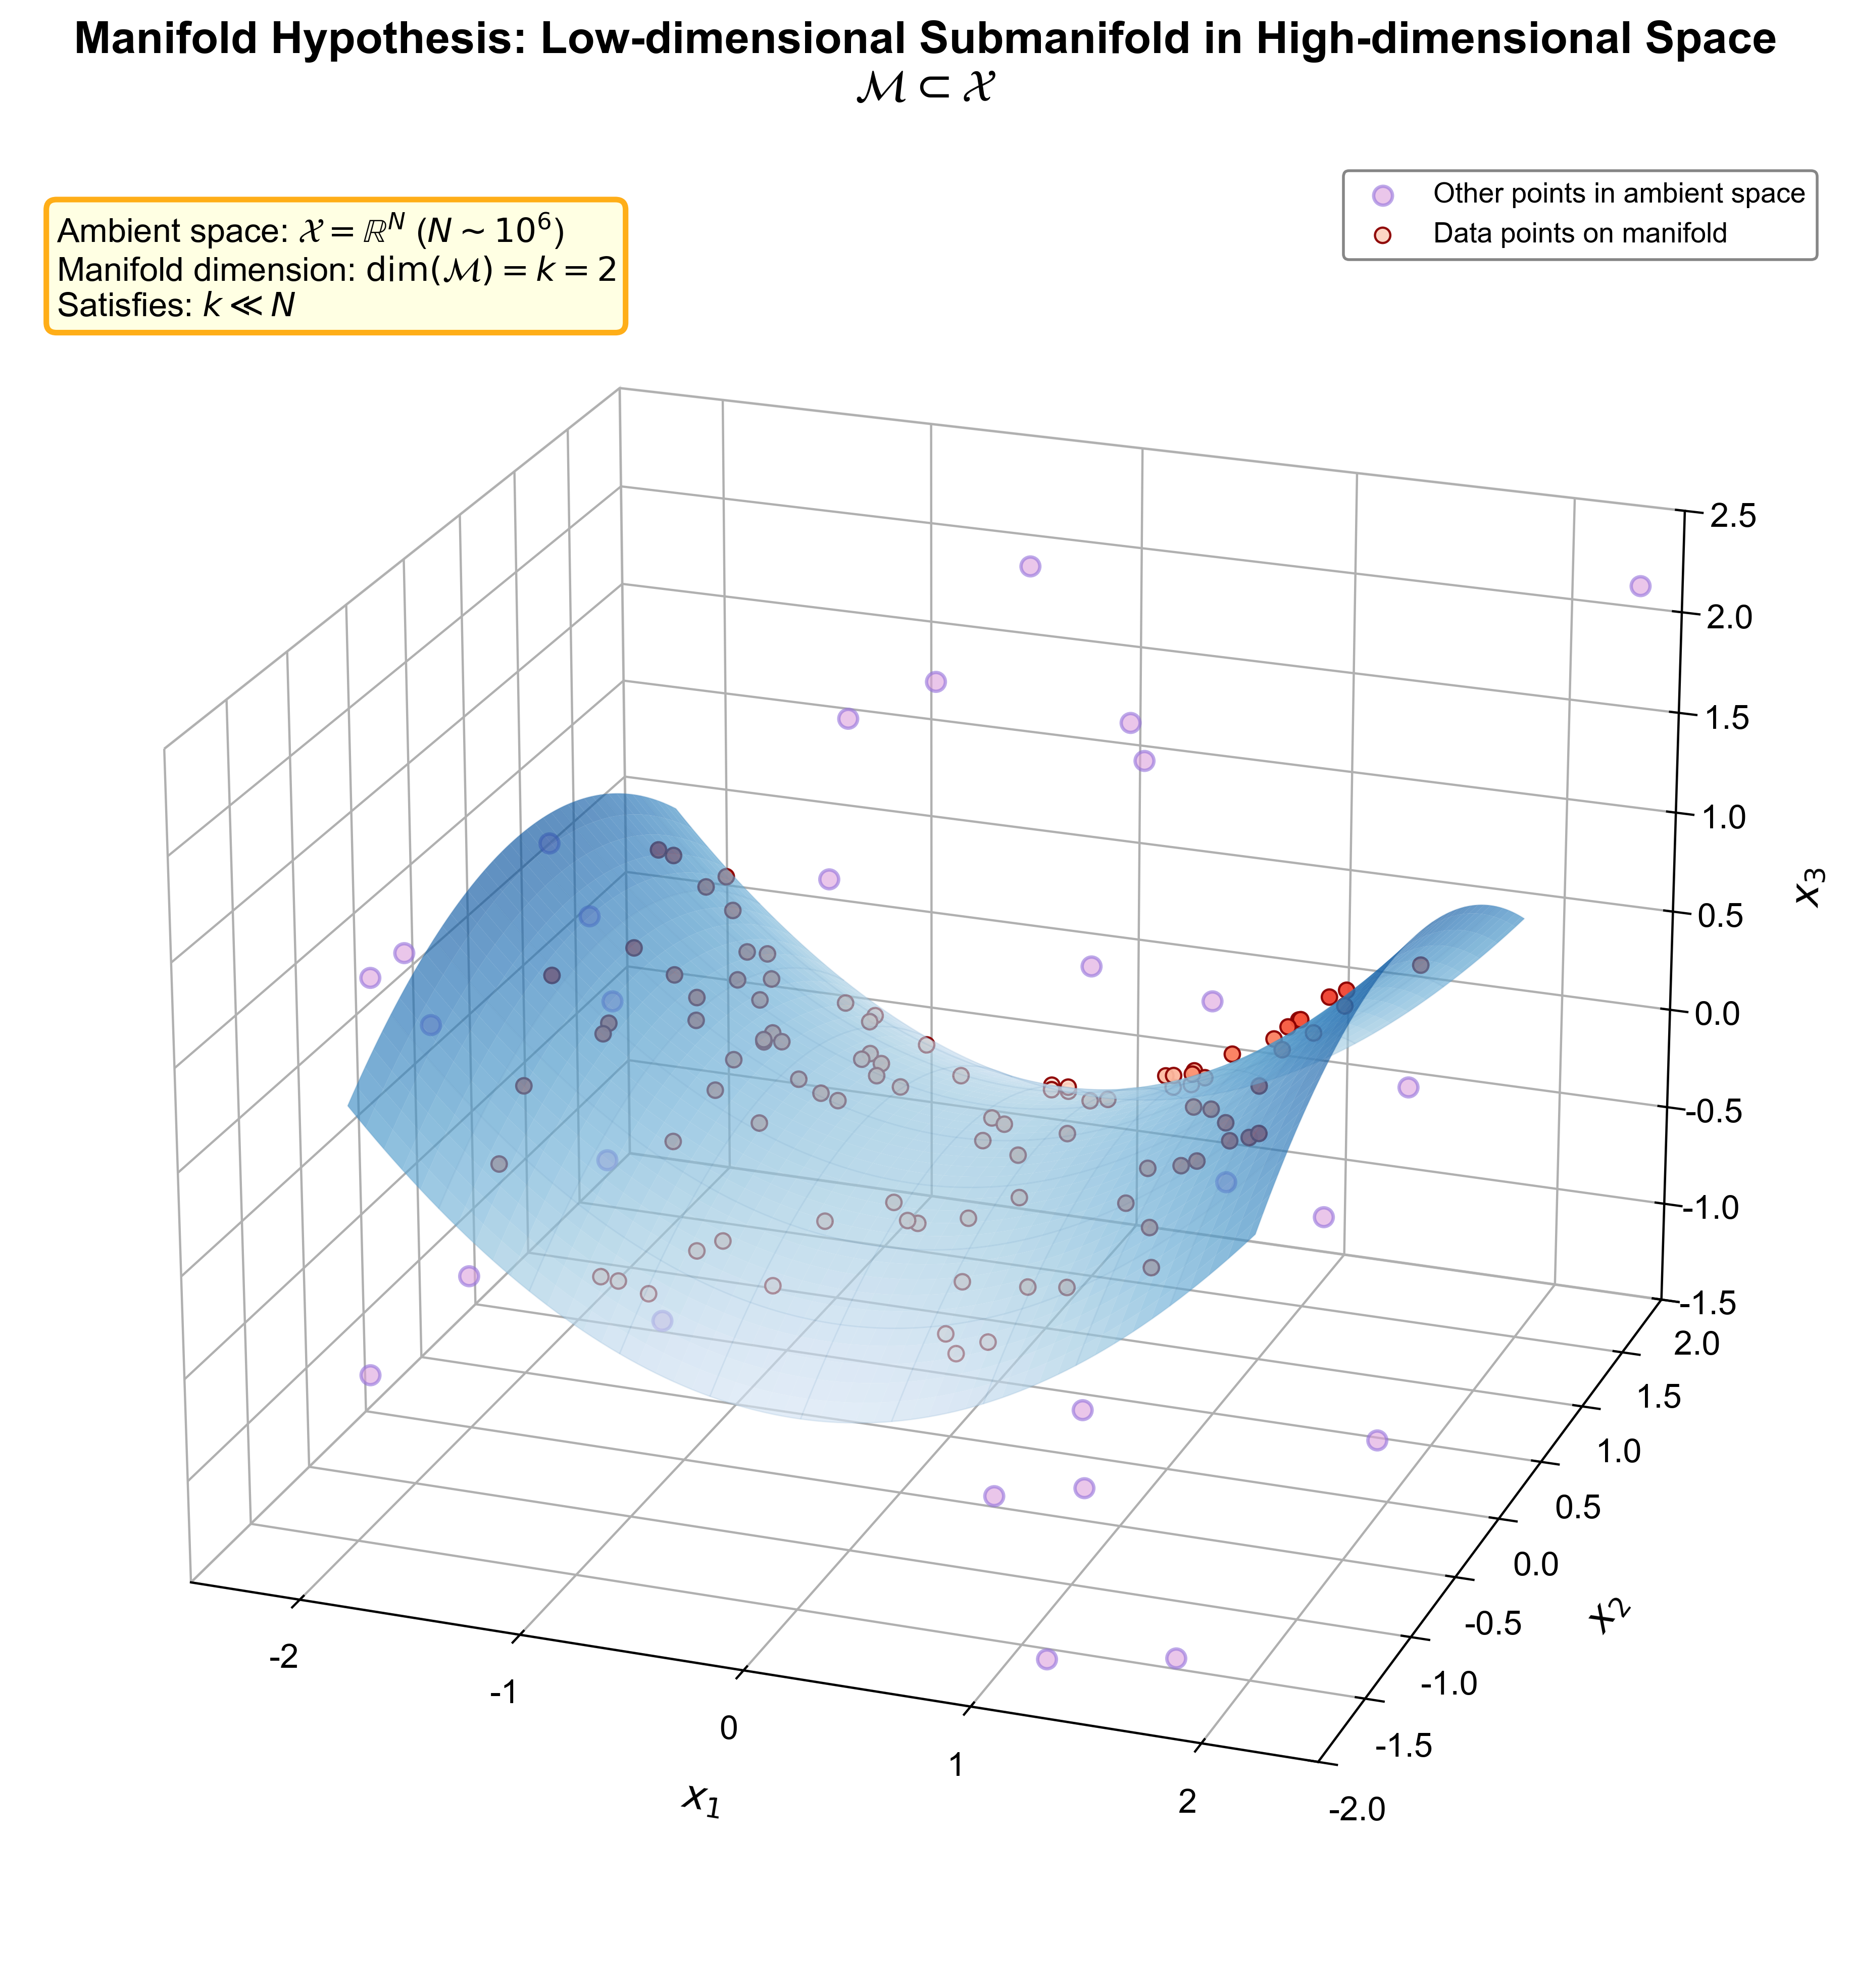
\includegraphics[width=1.00\textwidth]{./assets/manifold_hypothesis.png}
    \caption{流形假设的几何图景。红色点代表观测数据，集中在蓝色曲面 (流形 $\manifold$) 上。紫色点代表环境空间 $\dataspace$ 中的其他点，不在流形上，对应物理上不可实现的状态。}
    \label{fig:manifold_hypothesis}
\end{figure}

经验正交函数 (EOF) 是气候学中最常用的降维方法 \cite{hasselmann1988pips}。
对协方差矩阵 $\bm{C} = \frac{1}{n}\sum_{i=1}^n (\fastvar_i - \bar{\fastvar})(\fastvar_i - \bar{\fastvar})^\top$ 进行特征值分解，前 $K$ 个主成分的累积方差贡献率为:
\begin{equation}
\label{eq:eof_variance_contribution}
    r_K = \frac{\sum_{i=1}^K \eigenval_i}{\sum_{i=1}^N \eigenval_i}
\end{equation}

对于全球大气场，研究发现当 $K \sim 100$ 时，$r_K > 90\%$ \cite{hasselmann1988pips}。
这暗示大气子流形的内在维度约为 $10^2\text{--}10^3$，远小于 $N \sim 10^6$。
对于海洋子流形，主成分对应于一些气候模态: ENSO (解释约40\%方差) \cite{trenberth1997definition}、北大西洋涛动NAO \cite{hurrell1995decadal}、太平洋年代际振荡PDO、北极涛动AO等。
这些模态实际上就是流形的“坐标轴”，它们张成了切空间 $T_p\manifold$，定义了流形在该点的内在几何结构。
不同模态之间的正交性反映了流形局部坐标系的正交选取。

EOF 的有效性验证了流形假设: 如果数据分布在低维流形上，协方差矩阵的秩将远小于 $N$，特征值将快速衰减。
前 $K$ 个主成分对应于流形的坐标方向，任意状态可近似表示为 $\fastvar \approx \bar{\fastvar} + \sum_{k=1}^K a_k \mode_k$，其中 $\{\mode_k\}$ 是主成分，$\{a_k\}$ 是模态系数。

从动力学角度看，物理约束通过快速调整过程持续将状态轨迹“拉回”流形 \cite{ghil2008climate}。
如果因为某种原因产生了偏离流形的状态 (如负湿度、非地转平衡)，快速调整过程 (声波、重力波、湍流混合) 会在短时间内将系统恢复至流形上。
因此，流形具有吸引性，它是动力系统演化的不变集。

慢变量 $\slowvar$ 改变时，约束本身发生变化，流形 $\manifold_{\slowvar}$ 将随之变化。
例如，$\text{CO}_2$ 的增加将改变辐射平衡，温度上升将导致饱和水汽压增加 (Clausius-Clapeyron 关系)，从而改变湿度的可实现范围。
这体现为流形在相空间中的“移动”或“变形”。
在极端情况下，流形的拓扑结构可能会发生突变。

\subsection{参数化随机动力学}
\label{sec:stochastic_dynamics}

在固定慢变量 $\slowvar$ 下，快变量 $\fastvar_t$ 的演化并不是确定性的。
受计算资源限制和观测不确定性的影响，次网格过程 (湍流、对流、云微物理等) 无法被精确模拟，只能使用参数化方案进行统计性描述。
因此，我们需要一个随机动力学框架来描述快变量的演化。

\begin{assumption}[参数化随机动力学]
\label{ass:stochastic_dynamics}
    快变量 $\fastvar_t \in \manifold$ 的演化遵循伊藤随机微分方程 (Itô SDE) \cite{pavliotis2014stochastic}:
    \begin{equation}
    \label{eq:sde}
        d\fastvar_t = \drift(\fastvar_t; \slowvar)\,dt + \diffop(\fastvar_t; \slowvar)\,d\wiener_t
    \end{equation}

    其中:
    \begin{itemize}
        \item $\drift: \manifold \to T\manifold$ 是漂移向量场 (Drift Vector Field)，描述可解析尺度的确定性动力学；
        \item $\wiener_t \in \R^d$ 是 $d$ 维标准维纳过程 (Wiener Process)，满足 $\E[d\wiener_t] = 0$，$\E[d\wiener_t d\wiener_t^\top] = I_d\,dt$；
        \item $\diffop: \manifold \to \mathcal{L}(\R^d, T\manifold)$ 是扩散算子 (Diffusion Operator)，将 $\wiener_t$ 线性映射为切空间中的随机扰动；
        \item $\difftensor(\fastvar; \slowvar) = \diffop(\fastvar; \slowvar)\diffop(\fastvar; \slowvar)^\top \in \R^{N \times N}$ 是扩散张量 (Diffusion Tensor)，对称正定，描述随机扰动的协方差结构。
    \end{itemize}
\end{assumption}

我们逐个解释 Itô SDE 中各项的物理意义 (参见图 \ref{fig:ito_sde}):

\begin{figure}[htbp]
    \centering
    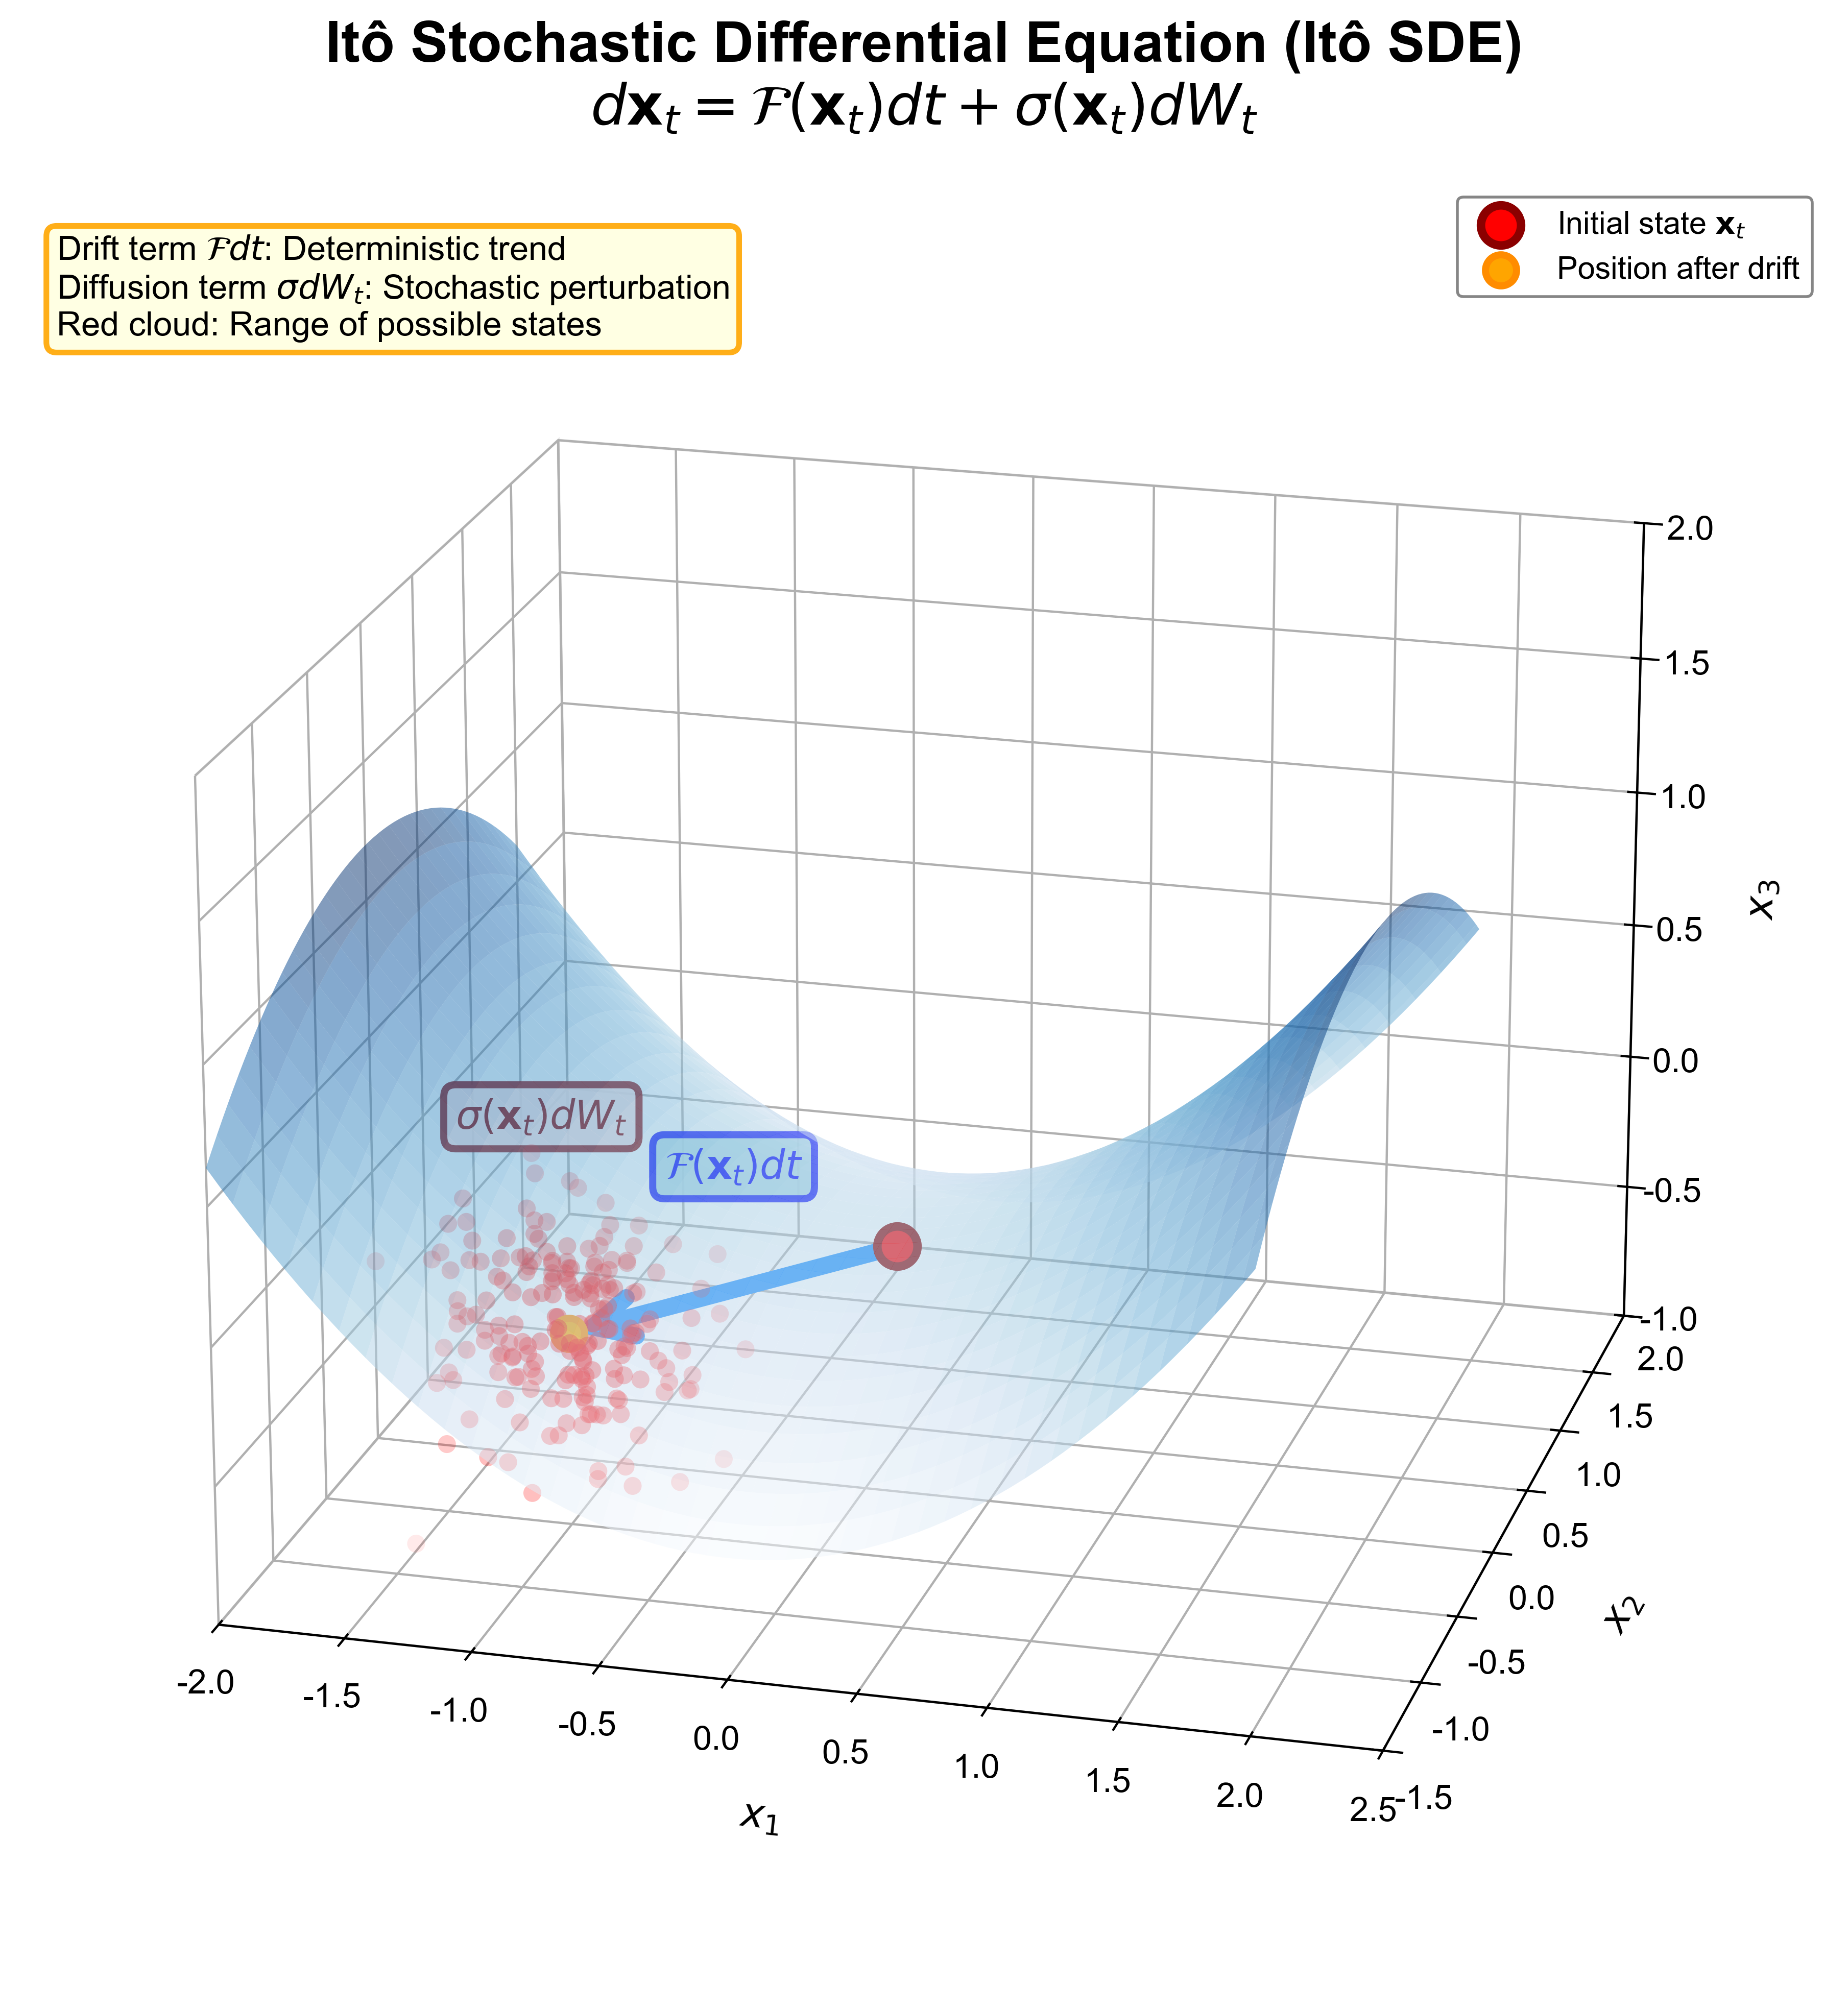
\includegraphics[width=1.00\textwidth]{./assets/ito_sde_visualization.png}
    \caption{伊藤随机微分方程的几何图景。红色点为初始状态 $\fastvar_t$，蓝色箭头为确定性漂移 $\drift(\fastvar_t)dt$，红色云团为随机扩散 $\diffop(\fastvar_t)d\wiener_t$ 产生的可能状态范围。橙色点为经过漂移后的状态。}
    \label{fig:ito_sde}
\end{figure}

\textbf{(1) 漂移项 $\drift(\fastvar; \slowvar)$}: 表示网格尺度可解析的物理过程，以及通过参数化方案统计性解析的次网格过程的系统性影响。
例如，在大气模式中，漂移项包括辐射强迫、大尺度平流、地转风平衡等确定性过程，也包括对流参数化方案给出的平均加热率、湍流参数化方案给出的平均应力。
在海洋模式中，漂移项包括风应力驱动的环流、温盐环流、以及涡参数化方案给出的平均输送。

\textbf{(2) 扩散项 $\diffop(\fastvar; \slowvar)\,d\wiener_t$}: 表示次网格过程的随机波动。
单个对流单体、湍流涡旋的生消是混沌的，无法显式跟踪。
在排除系统性影响 (已体现在漂移项) 后，我们可以用随机扩散描述其概率分布。
扩散张量 $\difftensor(\fastvar; \slowvar)$ 的对角元 $\difftensor_{ii}$ 表示第 $i$ 个自由度的随机扰动强度，非对角元 $\difftensor_{ij}$ 表示不同自由度的随机扰动相关性。
$\difftensor$ 的特征值和特征向量反映了随机扰动的主方向和强度。

\textbf{(3) 维纳过程的维度 $d$}: $d$ 是独立随机源的数量，可理解为主导的随机模态数 (如不同波数的湍流模态)。
扩散算子 $\diffop \in \R^{N \times d}$ 将 $d$ 维随机源映射为 $N$ 维状态扰动，通常 $d \ll N$。
这意味着随机扰动同样具有低维结构: 虽然状态空间是高维的，但驱动随机性的独立源数量有限。

方程 \eqref{eq:sde} 定义了一个马尔可夫过程 (Markov Process): 未来演化只依赖当前状态 $\fastvar_t$，与过去路径无关。
这假定了扩散项的记忆时间远小于漂移项的演化时间，即认为随机扰动无自相关 (白噪声近似)。
物理上，这要求次网格过程的相关时间 (湍流涡旋的寿命、对流单体的持续时间) 远小于大尺度演化的特征时间。
对于大气湍流 ($\sim$ 分钟)，相对于天气系统 ($\sim$ 天)，这一假设是合理的。
但对于某些中尺度过程 (如对流组织化)，可能需要考虑记忆效应，引入分数布朗运动、记忆核等非马尔可夫模型。

\vspace{1em}

我们建立的描述地球系统演化的随机动力学框架与Hasselmann \cite{hasselmann1976stochastic} 的开创性工作有着深刻的联系。
Hasselmann最早提出，快变量 (如大气湍流、对流) 对慢变量 (如海表温度) 的影响可以分解为两部分: 系统性的平均效应和随机的涨落效应。
他以此为基础构建了随机气候模型，成功解释了气候系统的红噪声谱特征，即气候变率的能量集中在低频段 \cite{hasselmann1976stochastic}。

然而，Hasselmann的原始工作主要基于物理直觉，缺乏严格的数学框架。
而现在，通过时间尺度分离、流形假设、Itô SDE等工具，我们可以将Hasselmann的随机气候模型纳入一个统一、严格的数学框架中。
方程 \eqref{eq:sde} 的漂移项 $\drift(\fastvar; \slowvar)$ 即对应于Hasselmann模型中的平均效应，扩散项 $\diffop(\fastvar; \slowvar)\,d\wiener_t$ 则对应于随机涨落。
更重要的是，我们明确了状态空间的流形结构 $\manifold$，将Hasselmann的线性随机模型推广到了非线性流形上，从而可以描述地球系统的几何结构。

\newpage

\section{Fokker-Planck方程与概率测度}
\label{sec:sde_measure}

由 \eqref{eq:sde} 定义的马尔可夫过程，其转移概率密度 $\probdens(\fastvar_t | \fastvar_0)$ 的演化满足\textbf{Fokker-Planck方程} \cite{gardiner2009stochastic}。
这一方程描述了概率密度在状态空间中的“流动”，是联系随机轨迹 (微观) 与概率分布 (宏观) 的桥梁。

\begin{theorem}[Fokker-Planck方程]
\label{thm:fp}
    设 $\probdens(\fastvar_t | \fastvar_0)$ 是从初始状态 $\fastvar_0$ 出发，在时刻 $t$ 位于 $\fastvar$ 的概率密度函数，则:
    \begin{equation}
    \label{eq:fp}
        \frac{\partial \probdens}{\partial t} = -\sum_{i=1}^N \frac{\partial}{\partial x_i}(\drift_i(\fastvar; \slowvar) \probdens) + \frac{1}{2}\sum_{i,j=1}^N \frac{\partial^2}{\partial x_i \partial x_j}(\difftensor_{ij}(\fastvar; \slowvar) \probdens)
    \end{equation}

    其中 $\drift_i$ 是漂移向量场的第 $i$ 个分量，$\difftensor_{ij} = [\diffop\diffop^\top]_{ij}$ 是扩散张量的分量。
\end{theorem}

从Itô SDE出发，对任意测试函数 $\phi(\fastvar)$ 应用期望算子，然后对测试函数作分部积分，
即得 \eqref{eq:fp}。
完整证明见 \cite{pavliotis2014stochastic}。

方程 \eqref{eq:fp} 具有清晰的物理意义清晰，概率密度的时间演化由两项驱动:
\begin{itemize}
    \item (漂移项) $-\sum_{i=1}^N \frac{\partial}{\partial x_i}(\drift_i(\fastvar; \slowvar) \probdens)$ 是\textbf{平流效应 (Advection)}，概率云被确定性向量场 $\drift$ 推动，如同流体中的质点随流场运动。
    \item (扩散项) $\frac{1}{2}\sum_{i,j} \frac{\partial^2}{\partial x_i \partial x_j}(\difftensor_{ij}(\fastvar; \slowvar) \probdens)$ 是\textbf{扩散效应 (Diffusion)}，概率云因随机扰动而展宽，如同热扩散中的温度弥散。
\end{itemize}

两者共同决定了概率密度的长期演化行为。
在足够长的时间后，如果系统满足遍历性条件，概率密度将趋于稳态，不再随时间变化。
这一稳态概率密度 $\probdens_{ss}(\fastvar; \slowvar)$ 满足稳态Fokker-Planck方程:

\begin{assumption}[稳态测度的存在性]
\label{ass:stationary_measure}
    对固定的 $\slowvar$，假设 SDE \eqref{eq:sde} 存在唯一的不变概率测度 $\measure_{\slowvar}$，其密度 $\probdens_{ss}(\fastvar; \slowvar)$ 满足稳态 Fokker-Planck 方程:
    \begin{equation}
    \label{eq:steady_fp}
        \frac{\partial \probdens_{ss}}{\partial t} = -\sum_{i=1}^N \frac{\partial}{\partial x_i}(\drift_i(\fastvar; \slowvar) \probdens_{ss}) + \frac{1}{2}\sum_{i,j=1}^N \frac{\partial^2}{\partial x_i \partial x_j}(\difftensor_{ij}(\fastvar; \slowvar) \probdens_{ss}) = 0
    \end{equation}
\end{assumption}

稳态方程 \eqref{eq:steady_fp} 表明，在稳态下，平流效应和扩散效应达到精确平衡: 向量场将概率密度推向某些区域，而扩散将其散布到更广的范围，两者的净效应相互抵消，概率分布保持不变。
这一平衡态即为\textbf{气候 (Climate)} 的数学定义——它是随机轨迹 (天气) 的长期统计性质。

\begin{definition}[概率测度]
\label{def:probability_measure}
    对固定的 $\slowvar$，概率测度 $\measure_{\slowvar}$ 由稳态密度 $\probdens_{ss}(\fastvar; \slowvar)$ 定义:
    \begin{equation}
    \label{eq:probability_measure}
        \measure_{\slowvar}(A) = \int_A \probdens_{ss}(\fastvar; \slowvar)\,d\fastvar, \quad \forall A \in \borel(\manifold)
    \end{equation}

    其中 $\borel(\manifold)$ 是流形的 Borel $\sigma$-代数。
\end{definition}

\begin{assumption}[遍历性]
\label{ass:ergodicity}
    假设马尔可夫过程 $\{\fastvar_t\}$ 在不变概率测度 $\measure_{\slowvar}$ 下是遍历的，即对任意可测函数 $\climind: \manifold \to \R$:
    \begin{equation}
    \label{eq:ergodic}
        \lim_{T \to \infty} \frac{1}{T}\int_0^T \climind(\fastvar_t)\,dt = \int_{\manifold} \climind(\fastvar)\,d\measure_{\slowvar}(\fastvar), \quad \text{几乎处处成立}
    \end{equation}
\end{assumption}

遍历性保证了时间平均和空间平均的等价性，是统计力学的基石 \cite{eckmann1985ergodic}。
想象一个粒子在流形 $\manifold$ 上遵循 Itô SDE \eqref{eq:sde} 进行随机游走。
给定足够长的时间，粒子会“走遍”流形的每个位置，在任意区域 $A$ 停留的时间比例 $\approx \measure_{\slowvar}(A)$。
除了零测集外，不存在粒子“永远无法到达”或“永远困在其中”的区域。
这意味着，长时间的观测可以充分采样概率测度，单个轨迹的时间平均可以代表集合平均。

在地球系统科学研究中，我们通常只能获得一条时间序列——比如某个气象站40年的逐日温度记录。
遍历性告诉我们: 这一条长时间序列的统计量 (如均值、方差) 趋近于真实的气候态，即温度的概率分布。
也就是说，\textbf{我们可以用对系统的长时间观察代替随机采样}。
这为从有限观测数据中推断地球系统的统计性质和气候学研究提供了理论保证。

遍历性假设在如下充分条件下可被严格证明 \cite{hairer2006ergodic}:
\begin{enumerate}
    \item 一致椭圆性: 扩散张量 $\difftensor(\fastvar; \slowvar)$ 处处非退化，即 $\exists \eigenval_{\min} > 0$ 使得 $\bm{\xi}^\top \difftensor(\fastvar; \slowvar) \bm{\xi} \geq \eigenval_{\min} \|\bm{\xi}\|^2$ 对所有 $\fastvar \in \manifold$ 和 $\bm{\xi} \in \R^N$ 成立；
    \item 次线性增长条件: $\exists C > 0$ 使得 $\|\drift(\fastvar; \slowvar)\| \leq C(1 + \|\fastvar\|)$ 对所有 $\fastvar \in \manifold$ 成立；
    \item 耗散性: $\exists \alpha, \beta > 0$ 使得 $\langle \drift(\fastvar; \slowvar), \fastvar \rangle \leq -\alpha \|\fastvar\|^2 + \beta$ 对充分大的 $\|\fastvar\|$ 成立。
\end{enumerate}

对于地球系统而言，这些条件在物理上具有合理性: 条件 (1) 要求次网格随机扰动处处非零 (湍流、对流过程无处不在); 条件 (2) 要求物理量不会无限增长 (温度、风速存在能量上界约束); 条件 (3) 要求存在能量耗散机制 (摩擦、辐射冷却、边界层拖曳)。
因此，我们认为遍历性假设在地球系统中是成立的。

\newpage

\section{度量张量}
\label{sec:metric_tensor}

在 \ref{sec:earth_system} 章中，我们认为地球系统是流形上的随机动力学过程。
为了更加深入地分析地球系统的几何结构，我们需要在流形 $\manifold$ 上定义距离、角度、体积、曲率等几何概念。
我们希望取得一个良好的定义，使得这些几何概念能够尽量充分地反映动力学过程的信息。

定义\textbf{度量张量 (Metric Tensor)} $\metric$。

\begin{definition}[度量张量]
\label{def:metric_tensor}
    度量张量 $g$ 是定义在流形切丛上的一个光滑、对称、正定的 $(0, 2)$ 型张量场。在局部坐标 $\bm{u} = (u^1, \ldots, u^k)$ 下，它表示为对称正定矩阵 $[\metric_{ij}(\bm{u})]$。
    两个无穷接近的点之间的距离平方为:
    \begin{equation}
    \label{eq:metric_tensor_def}
        ds^2 = \sum_{i,j=1}^k g_{ij}(\bm{u})\,du^i\,du^j = d\bm{u}^\top \metric(\bm{u}) d\bm{u}
    \end{equation}
\end{definition}

基于度量张量 $\metric$，我们定义\textbf{测地距离 (Geodesic Distance)} $d_\metric$。

\begin{definition}[测地距离]
\label{def:geodesic_distance}
    给定度量张量 $\metric$，流形 $\manifold$ 上两点 $p, q$ 之间的测地距离 $d_\metric(p, q)$ 定义为:
    \begin{equation}
    \label{eq:geodesic_distance}
        d_\metric(p, q) = \inf_{\gamma: p \to q} \int_0^1 \sqrt{\sum_{i,j=1}^k \metric_{ij}(\gamma(t)) \dot{\gamma}^i(t) \dot{\gamma}^j(t)}\, dt
    \end{equation}

    其中 $\gamma: [0,1] \to \manifold$ 是连接 $p = \gamma(0)$ 和 $q = \gamma(1)$ 的光滑曲线，$\dot{\gamma}(t) = \frac{d\gamma}{dt}$ 是切向量。
    测地距离是所有连接 $p$ 和 $q$ 的曲线中最短的弧长。
\end{definition}

我们定义\textbf{曲率 (Curvature)} 来刻画流形的弯曲程度 \cite{lee2018introduction}。

\begin{definition}[Riemann曲率张量]
\label{def:riemann_curvature_tensor}
    \begin{equation}
    \label{eq:riemann_curvature_tensor}
        R_{ijkl} = \frac{\partial \Gamma_{il}^m}{\partial x^k} - \frac{\partial \Gamma_{ik}^m}{\partial x^l} + \Gamma_{il}^n\Gamma_{nk}^m - \Gamma_{ik}^n\Gamma_{nl}^m
    \end{equation}

    其中 $\Gamma_{jk}^i = \frac{1}{2}g^{im}(\frac{\partial g_{mj}}{\partial x^k} + \frac{\partial g_{mk}}{\partial x^j} - \frac{\partial g_{jk}}{\partial x^m})$ 是Christoffel符号。
\end{definition}

通过对Riemann曲率张量进行收缩，可得到Ricci曲率张量: $\mathrm{Ric}_{ij} = R_{ikjl}g^{kl}$。
进一步收缩，得到\textbf{标量曲率}: $R = \mathrm{Ric}_{ij}g^{ij}$。
标量曲率 $R$ 可近似理解为度量张量的二阶变化:
\begin{equation}
\label{eq:scalar_curvature_approximation}
    R \sim \|\nabla^2 g\|
\end{equation}

标量曲率的符号反映了流形局部的凹凸性: 正曲率表示“碗状”，负曲率对应“鞍状”，零曲率对应平坦区域。

\subsection{近邻假设}

\textbf{近邻假设 (Neighborhood Preserving)} 认为: \textbf{在流形上距离相近的点，其演化行为应该是类似的} (参见图 \ref{fig:neighborhood_preserving})。
考虑演化算子 $\evolop_t: \manifold \to \manifold$，$\evolop_t(\fastvar_0) = \fastvar(t)$。
一个好的度量 $\dyndist_\metric$ 应使 $\evolop_t$ 具有小的Lipschitz常数 $L$:
\begin{equation}
\label{eq:neighborhood_preserving}
    \dyndist_\metric(\evolop_t(\fastvar_A), \evolop_t(\fastvar_B)) \leq L \cdot \dyndist_\metric(\fastvar_A, \fastvar_B), \quad \forall \fastvar_A, \fastvar_B \in \manifold
\end{equation}

\begin{figure}[htbp]
    \centering
    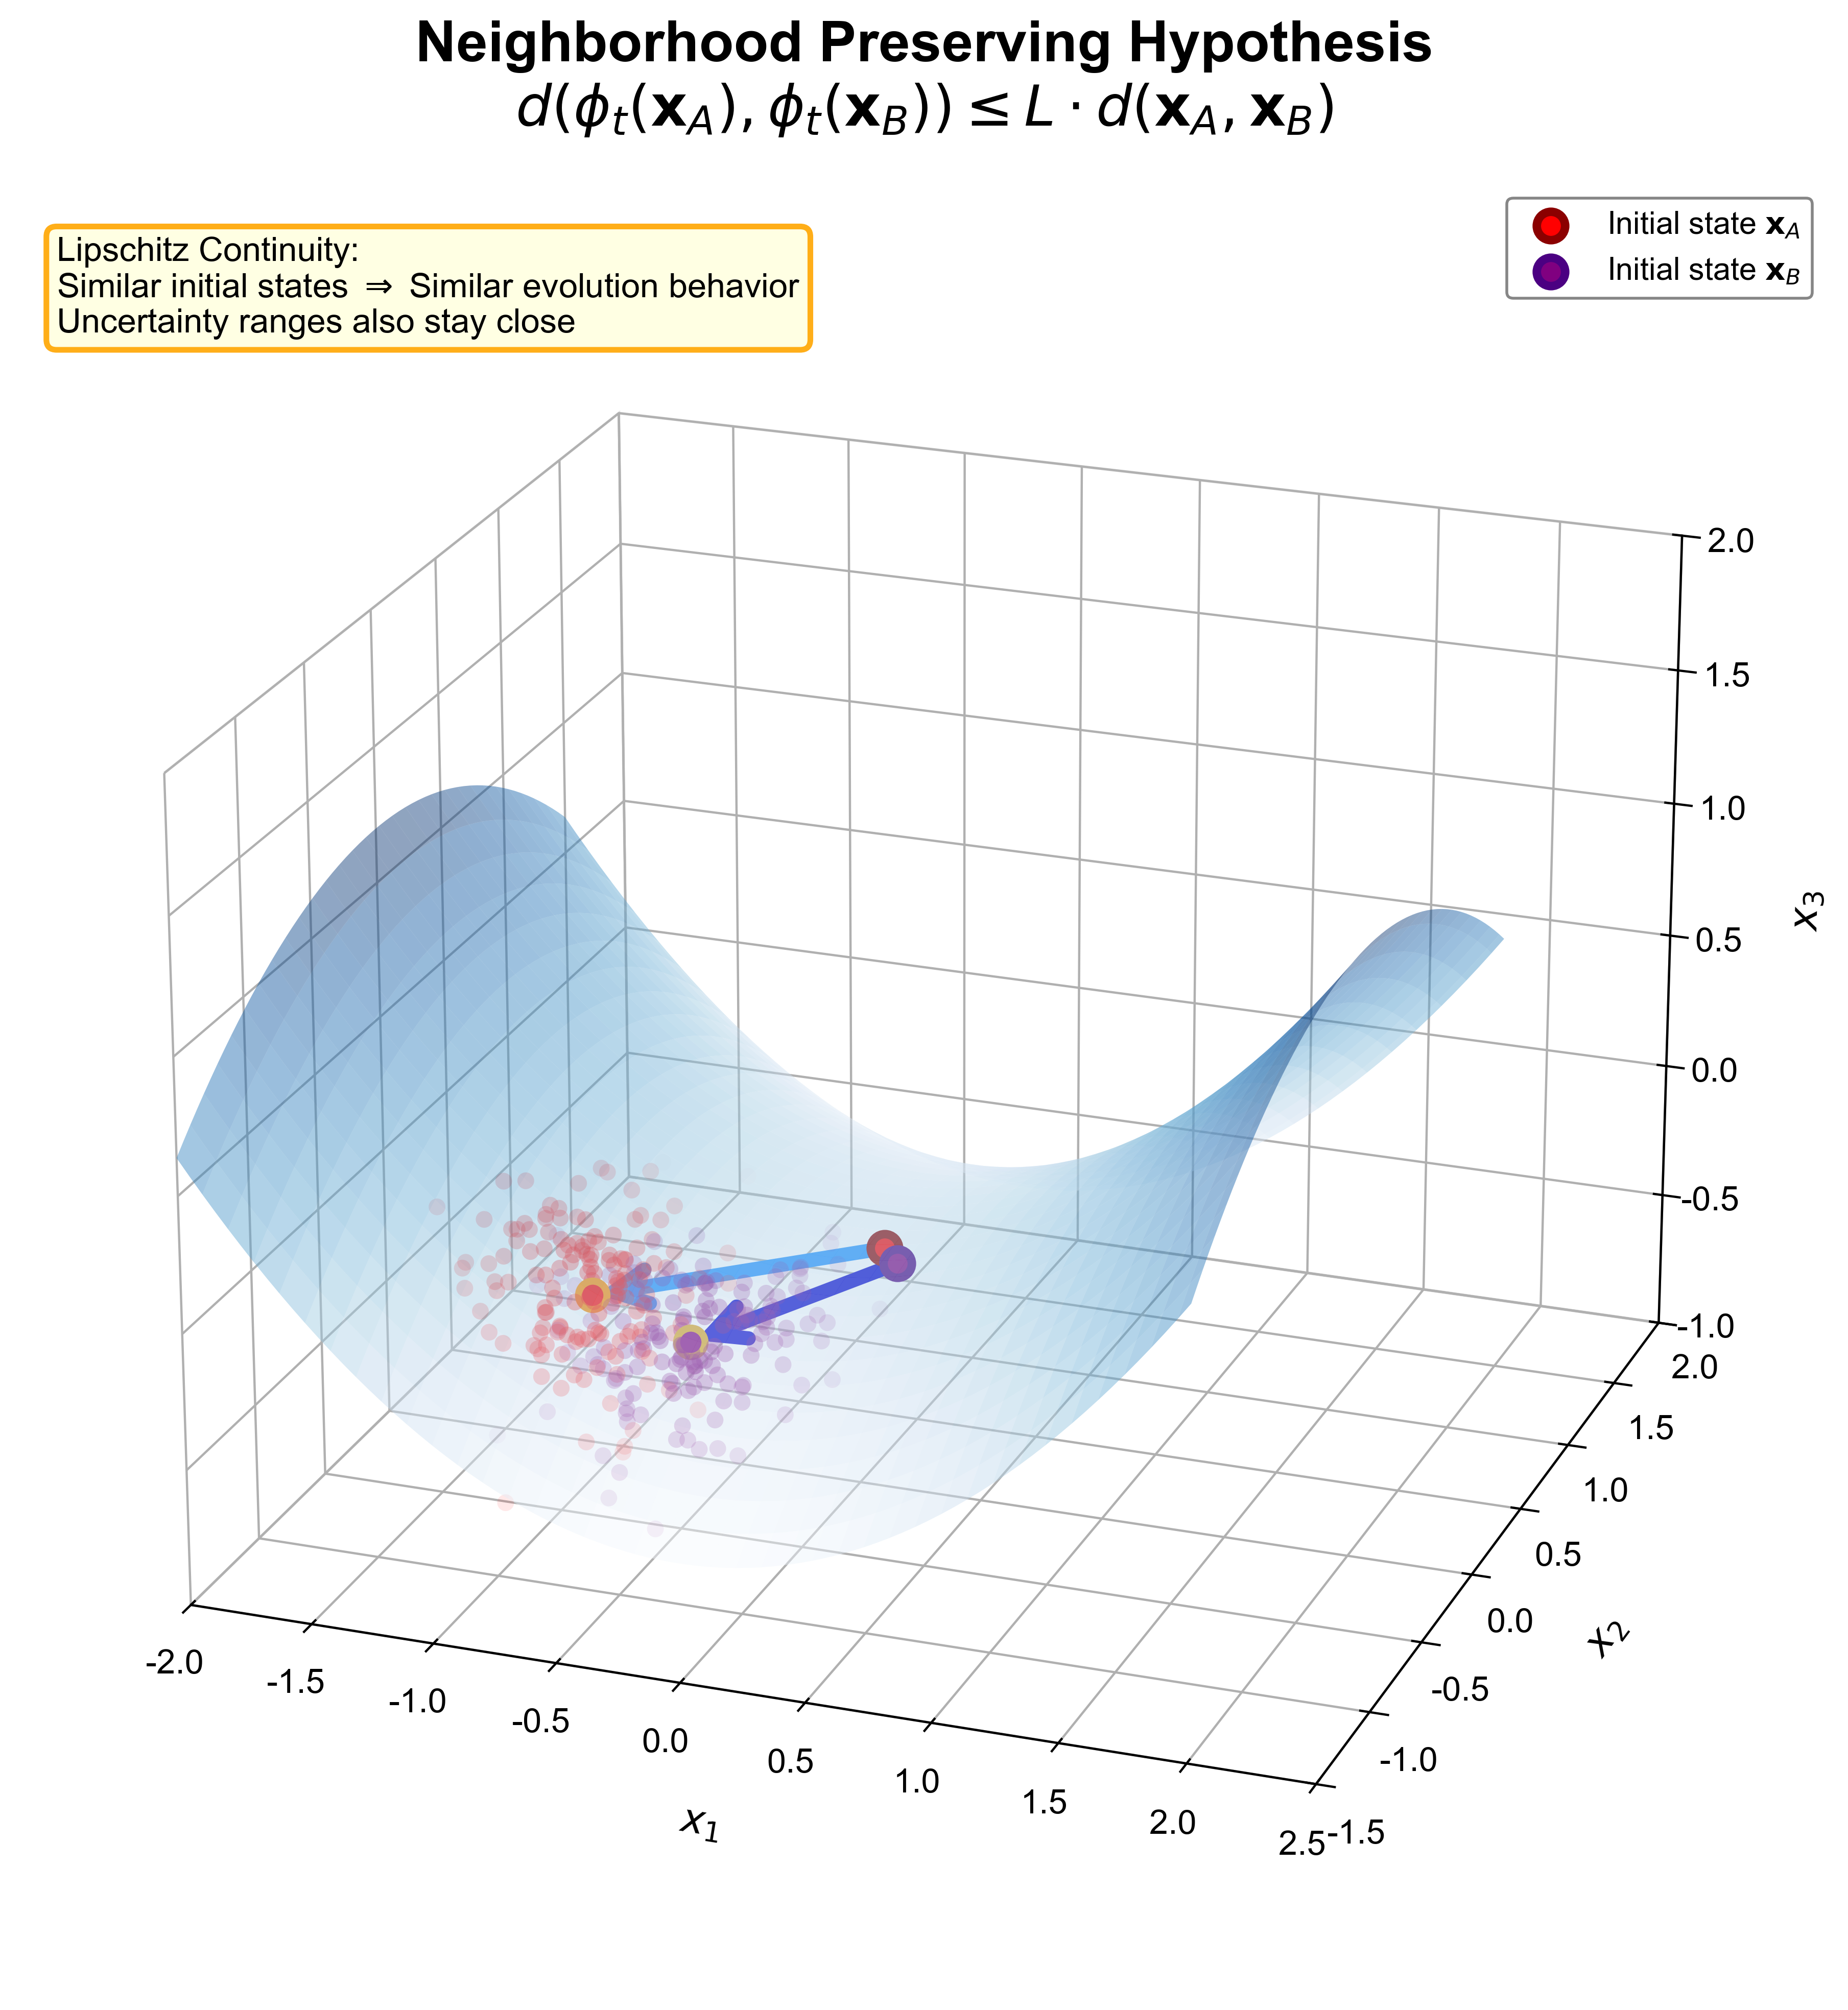
\includegraphics[width=1.00\textwidth]{./assets/neighborhood_preserving.png}
    \caption{近邻假设的几何图景。红色和紫色点代表两初始状态 $\fastvar_A, \fastvar_B$，蓝色和紫色箭头为各自的漂移方向，红色和紫色云团为各自的扩散范围。近邻假设要求: 若初始状态接近，则未来状态的概率分布也应相似。}
    \label{fig:neighborhood_preserving}
\end{figure}

在尝试拟合演化算子 $\evolop_t$ 时，Lipschitz平滑性 \eqref{eq:neighborhood_preserving} 将带来以下好处:
\begin{itemize}
    \item 稳定性 (Stability): 模型具有更高的可预报性极限；
    \item 泛化性 (Generalization): 模型在训练样本的“近邻”内泛化误差可控，预测可靠性高；
    \item 正则化 (Regularization): 较小的Lipschitz常数隐含正则化条件，可以防止模型过拟合；
    \item 鲁棒性 (Robustness): 模型能够容忍一定的观测误差和数值误差。
\end{itemize}

因此，如何构造符合近邻假设，具有较好Lipschitz平滑性的度量 $\metric$，是一个十分重要的问题。
欧氏距离 $\dyndist_{\text{Euclid}}(\fastvar_A, \fastvar_B) = \|\fastvar_A - \fastvar_B\|_2$ 显然不是一个好的选择——物理上相似的状态在欧氏距离下可能很远，物理上差异巨大的状态反而接近。
这里举一个具体例子，我们考虑两个扰动:
\begin{itemize}
    \item 扰动A: ENSO核心区 (约占全球面积的 1\%) 的0.5K海温异常。
    \item 扰动B: 全球每个格点均匀的0.01K温度扰动。
\end{itemize}

按照欧式距离，扰动B的影响更大，即扰动前后状态的距离更远，相似性更低。
但从气候动力学角度理解: 扰动A会在数周内通过Walker环流以遥相关的方式影响全球天气，而扰动B几乎不会产生任何影响。
这说明欧氏距离给出了错误的相似性判断。
如果我们基于此进行建模，模型会认为扰动B的效果“更显著”，这与物理实际完全相反。

\subsection{动力学距离}

Itô SDE \eqref{eq:sde} 描述的动力学系统是随机的。
从初始状态 $\fastvar_0$ 出发，系统在未来 $\predtime$ 时刻的状态 $\fastvar_{\predtime}$ 服从概率分布 $\probdens_{\predtime}(\cdot | \fastvar_0)$。
根据近邻保持假设，\textbf{动力学相似性应由未来状态分布的差异来衡量}。

\begin{definition}[动力学距离]
\label{def:tau_distance}
    固定预报时间 $\predtime > 0$，两初值 $\fastvar_A, \fastvar_B$ 的动力学距离定义为:
    \begin{equation}
    \label{eq:tau_distance}
        d_{\predtime}(\fastvar_A, \fastvar_B) = \sqrt{\predtime} \cdot d_p(\probdens_{\predtime}(\cdot | \fastvar_A), \probdens_{\predtime}(\cdot | \fastvar_B))
    \end{equation}

    其中 $d_p$ 是量化概率分布差异的距离函数，如 Wasserstein 距离 \cite{villani2009optimal}。
    时间权重因子 $\sqrt{\predtime}$ 反映了预报时间对距离度量的自然贡献。
\end{definition}

为推导 $d_{\predtime}$ 的显式形式，需要分析\textbf{SDE的有限时间演化}。
考虑相邻初值 $\fastvar_A, \fastvar_B$，记 $\delta\fastvar_0 = \fastvar_B - \fastvar_A$ 为初始扰动。
我们需要一系列简化假设来使问题在数学上可处理。

\begin{assumption}[局部平稳扩散]
\label{ass:local_stationary_diffusion}
    扩散算子 $\diffop(\fastvar)$ 在小邻域内近似常数:
    \begin{equation}
    \label{eq:local_stationary_diffusion}
        \diffop(\fastvar+\delta\fastvar) \approx \diffop(\fastvar)
    \end{equation}
\end{assumption}

\begin{assumption}[局部线性化]
\label{ass:local_linearization}
    在初值的小邻域 $\|\delta\fastvar_0\|$ 内，漂移项可线性化:
    \begin{equation}
    \label{eq:local_linearization}
        \drift(\fastvar + \delta\fastvar) \approx \drift(\fastvar) + \jacobian_{\drift}(\fastvar) \delta\fastvar
    \end{equation}

    其中 $\jacobian_{\drift} = \frac{\partial \drift}{\partial \fastvar}$ 是雅可比矩阵。
\end{assumption}

\begin{assumption}[适度时间尺度]
\label{ass:moderate_time_scale}
    预报时间 $\predtime$ 满足:
    \begin{equation}
    \label{eq:moderate_time_scale}
        \predtime \ll \frac{1}{\|\jacobian_{\drift}\|} \cdot \frac{L_{\drift}}{\|\delta\fastvar_0\|}
    \end{equation}

    其中 $L_{\drift}$ 是系统特征尺度。这保证线性近似在 $[0, \predtime]$ 内有效。
\end{assumption}

\begin{assumption}[缓变场假设]
\label{ass:slowly_varying_fields}
    雅可比矩阵 $\jacobian_{\drift}(\fastvar_t)$ 和扩散算子 $\diffop(\fastvar_t)$ 在时间尺度 $\predtime$ 内近似常数:
    \begin{equation}
    \label{eq:slowly_varying_fields}
        \jacobian_{\drift}(\fastvar_t) \approx \jacobian_{\drift}(\fastvar_0), \quad \diffop(\fastvar_t) \approx \diffop(\fastvar_0), \quad \forall t \in [0, \predtime]
    \end{equation}
\end{assumption}

以上简化假设的核心思想是进行\textbf{局部时空小扰动近似}: 在空间上，我们假设在一个小邻域内，随机动力学过程的漂移项是线性的，扩散项是恒定的；在时间上，我们要求预报时间 $\predtime$ 相对较短，以至于线性近似依然有效，且动力学过程本身在此期间可视为“冻结”不变。
这些假设在特定条件下是合理的，例如在分析稳定背景场 (如长期气候平均态) 附近的、演化时间较短的小扰动时。

根据假设 \ref{ass:local_stationary_diffusion} 和 \ref{ass:local_linearization}，扰动的演化满足线性化SDE:
\begin{equation}
\label{eq:linearized_sde}
    d(\delta\fastvar_t) = \jacobian_{\drift}(\fastvar_t) \delta\fastvar_t\,dt + \diffop(\fastvar_t) d\wiener_t
\end{equation}

考虑从初值 $\fastvar_A$ 和 $\fastvar_B = \fastvar_A + \delta\fastvar_0$ 出发的两条轨迹。
在假设 \ref{ass:slowly_varying_fields} 下，线性化SDE \eqref{eq:linearized_sde} 是常系数的，其解为:
\begin{equation}
\label{eq:perturbation_solution}
    \delta\fastvar_t = \fundsol_t \delta\fastvar_0 + \int_0^t \fundsol_{t-s} \diffop d\wiener_s
\end{equation}

其中 $\fundsol_t = e^{\jacobian_{\drift}(\fastvar_0) t}$ 是基本解矩阵。
\eqref{eq:perturbation_solution} 表明扰动由动力学指数放大 ($\fundsol_t \delta\fastvar_0$) 和随机扰动累计 ($\int_0^t \fundsol_{t-s}\diffop d\wiener_s$) 两部分构成。

由 \eqref{eq:perturbation_solution} 决定的未来状态概率分布是高斯分布。
具体地，从 $\fastvar_A$ 出发的轨迹在时刻 $\predtime$ 的分布为:
\begin{equation}
\label{eq:gaussian_distribution_of_perturbation_A}
    \probdens_{\predtime}(\cdot|\fastvar_A) = \normdist(\bm{m}_A, \covmat_{\predtime})
\end{equation}

其中 $\bm{m}_A = \fastvar_A + \mathbb{E}\left[\int_0^{\predtime} \drift(\fastvar_A(s)) ds\right]$。
其中协方差为随机扰动的累积效应，根据Itô等距性质 $\mathbb{E}[d\wiener_s d\wiener_s^\top] = I ds$，有:
\begin{equation}
\label{eq:covariance_of_perturbation}
    \covmat_{\predtime} = \mathbb{E}\left[\left(\int_0^{\predtime} \fundsol_{\predtime-s}\diffop d\wiener_s\right) \left(\int_0^{\predtime} \fundsol_{\predtime-s}\diffop d\wiener_s\right)^\top\right] = \int_0^{\predtime} \fundsol_s \difftensor \fundsol_s^\top ds
\end{equation}

类似地，从 $\fastvar_B$ 出发的轨迹在时刻 $\predtime$ 的分布为:
\begin{equation}
\label{eq:gaussian_distribution_of_perturbation_B}
    \probdens_{\predtime}(\cdot|\fastvar_B) = \normdist(\bm{m}_B, \covmat_{\predtime})
\end{equation}

有 $\bm{m}_B = \fastvar_B + \mathbb{E}\left[\int_0^{\predtime} \drift(\fastvar_B(s)) ds\right]$。
注意到 $\probdens_{\predtime}(\cdot|\fastvar_A)$ 和 $\probdens_{\predtime}(\cdot|\fastvar_B)$ 的协方差相同，因为二者的随机扰动都来自标准Wiener过程。

我们取 $d_p(\probdens_{\predtime}(\cdot|\fastvar_A), \probdens_{\predtime}(\cdot|\fastvar_B)) = (\bm{m}_A - \bm{m}_B)^\top \covmat_{\predtime}^{-1} (\bm{m}_A - \bm{m}_B)$，用来描述两个概率分布的差异。
对于共享协方差矩阵的高斯分布，这等价于使用Mahalanobis距离或KL散度 (此时KL散度也是对称的)。

现在计算均值差。
在假设 \ref{ass:local_linearization}下，漂移项满足 $\drift(\fastvar_B(s)) - \drift(\fastvar_A(s)) \approx \jacobian_{\drift} \delta\fastvar_s$，因此:
\begin{align*}
    \bm{m}_B - \bm{m}_A &\approx \delta\fastvar_0 + \mathbb{E}\left[\int_0^{\predtime} \jacobian_{\drift} \delta\fastvar_s ds\right] \\
    &= \delta\fastvar_0 + \mathbb{E}\left[\int_0^{\predtime} \jacobian_{\drift} (\fundsol_s \delta\fastvar_0 + \int_0^s \fundsol_{s-s^\prime} \diffop d\wiener_{s^\prime}) ds\right] \\
    &= \delta\fastvar_0 + \int_0^{\predtime} \jacobian_{\drift} \fundsol_s \delta\fastvar_0 ds + \mathbb{E}\left[\int_0^{\predtime} \int_0^s \jacobian_{\drift} \fundsol_{s-s^\prime} \diffop d\wiener_{s^\prime} ds\right] \\
    &= \delta\fastvar_0 + (\fundsol_{\predtime} - \fundsol_0) \delta\fastvar_0 \\
    &= \fundsol_{\predtime} \delta\fastvar_0
\end{align*}

将均值差代入 \eqref{eq:tau_distance}:
\begin{equation}
\label{eq:tau_distance_final}
    \dyndist_{\predtime}^2(\fastvar_A, \fastvar_B) = \predtime \cdot \delta\fastvar_0^\top \fundsol_{\predtime}^\top \left(\int_0^{\predtime} \fundsol_s \difftensor \fundsol_s^\top ds\right)^{-1} \fundsol_{\predtime} \delta\fastvar_0
\end{equation}

根据定义 \eqref{eq:metric_tensor_def}，导出度量张量:
\begin{equation}
\label{eq:metric_tensor_final}
    \metric_{\predtime}(\fastvar) = \predtime \cdot \fundsol_{\predtime}^\top \left(\int_0^{\predtime} \fundsol_s \difftensor \fundsol_s^\top ds\right)^{-1} \fundsol_{\predtime}
\end{equation}

\subsection{渐近分析}

为理解预报时间 $\predtime$ 对系统几何结构的影响，我们分析度量张量在不同时间尺度下的渐近行为。
我们需要引入对称性与对角化假设，以进一步化简 \eqref{eq:metric_tensor_final}。

\begin{assumption}[对称性与对角化]
\label{ass:commuting_matrices}
    雅可比矩阵 $\jacobian_{\drift}$ 是对称矩阵 ($\jacobian_{\drift} = \jacobian_{\drift}^\top$)，且与扩散张量 $\difftensor$ 可交换 ($[\jacobian_{\drift}, \difftensor] = 0$)。在此条件下，存在正交矩阵 $\eigenvecmat$ 使得:
    \begin{equation}
    \label{eq:simultaneous_diagonalization}
        \jacobian_{\drift} = \eigenvecmat\eigenvalmat \eigenvecmat^\top, \quad \difftensor = \eigenvecmat\diffeigenvalmat \eigenvecmat^\top
    \end{equation}

    其中 $\eigenvalmat = \text{diag}(\eigenval_1, \ldots, \eigenval_N)$ 为实特征值矩阵，$\diffeigenvalmat = \text{diag}(\delta_1, \ldots, \delta_N)$ 为正特征值矩阵。
\end{assumption}

对称性假设要求动力学系统局部上可表示为梯度流 $\drift \approx -\nabla \Phi$，其中 $\Phi$ 是势函数。
这对应于无环流、纯耗散的系统。
在地球系统中，仅部分变量的子系统的雅可比矩阵近似对称，如海洋热含量、土壤湿度等；但对于存在环流、相位传播的子系统，如大气急流、Rossby波等，通常具有非对称的雅可比矩阵。
可交换性进一步要求动力学演化的主方向与随机扰动的主方向对齐，这在一定程度上是合理的，但并非总是成立。
因此，假设 \ref{ass:commuting_matrices} 是较强的简化，我们基于此假设的分析仅提供定性的洞察。

在假设 \ref{ass:commuting_matrices} 下，协方差矩阵 $\covmat_{\predtime}$ 具有简洁的对角化形式。
\begin{align*}
    \covmat_{\predtime} = \int_0^{\predtime} \fundsol_s \difftensor \fundsol_s^\top ds &= \int_0^{\predtime} \eigenvecmat e^{\eigenvalmat s} \eigenvecmat^\top \difftensor \eigenvecmat e^{\eigenvalmat^\top s} \eigenvecmat^\top ds \\
    &= \eigenvecmat \left(\int_0^{\predtime} e^{\eigenvalmat s} (\eigenvecmat^\top \difftensor \eigenvecmat) e^{\eigenvalmat^\top s} ds\right) \eigenvecmat^\top \\
    &= \eigenvecmat \left(\int_0^{\predtime} e^{\eigenvalmat s} \diffeigenvalmat e^{\eigenvalmat^\top s} ds\right) \eigenvecmat^\top \\
    &= \eigenvecmat \left(\text{diag}(\frac{\delta_i}{2 \eigenval_i} (e^{2 \eigenval_i \predtime} - 1))\right) \eigenvecmat^\top
\end{align*}

度量张量 $\metric_{\predtime}$ 为:
\begin{align*}
    \metric_{\predtime} = \predtime \cdot \fundsol_{\predtime}^\top \covmat_{\predtime}^{-1} \fundsol_{\predtime} &= \predtime \cdot \eigenvecmat e^{\eigenvalmat^\top \predtime} \eigenvecmat^\top \eigenvecmat \left(\text{diag}(\frac{\delta_i}{2 \eigenval_i} (e^{2 \eigenval_i \predtime} - 1))\right)^{-1} \eigenvecmat^\top \eigenvecmat e^{\eigenvalmat \predtime} \eigenvecmat^\top \\
    &= \predtime \cdot \eigenvecmat e^{\eigenvalmat^\top \predtime} \left(\text{diag}(\frac{2 \eigenval_i}{\delta_i} \frac{1}{e^{2\eigenval_i \predtime} - 1})\right) e^{\eigenvalmat \predtime} \eigenvecmat^\top \\
    &= \eigenvecmat \left(\text{diag}\left(\frac{2 \eigenval_i \predtime}{\delta_i} \frac{e^{2\eigenval_i \predtime}}{e^{2\eigenval_i \predtime} - 1}\right)\right) \eigenvecmat^\top
\end{align*}

度量对角元为:
\begin{equation}
\label{eq:metric_tensor_diagonal_element}
    [\metric_{\predtime}]_{ii} = \frac{2\eigenval_i \predtime}{\delta_i} \frac{e^{2\eigenval_i\predtime}}{e^{2\eigenval_i\predtime} - 1}
\end{equation}

图 \ref{fig:metric_vs_tau} 展示了不同 $\eigenval_i$ 取值下度量对角元随预报时间 $\predtime$ 的演化。
\begin{figure}[htbp]
    \centering
    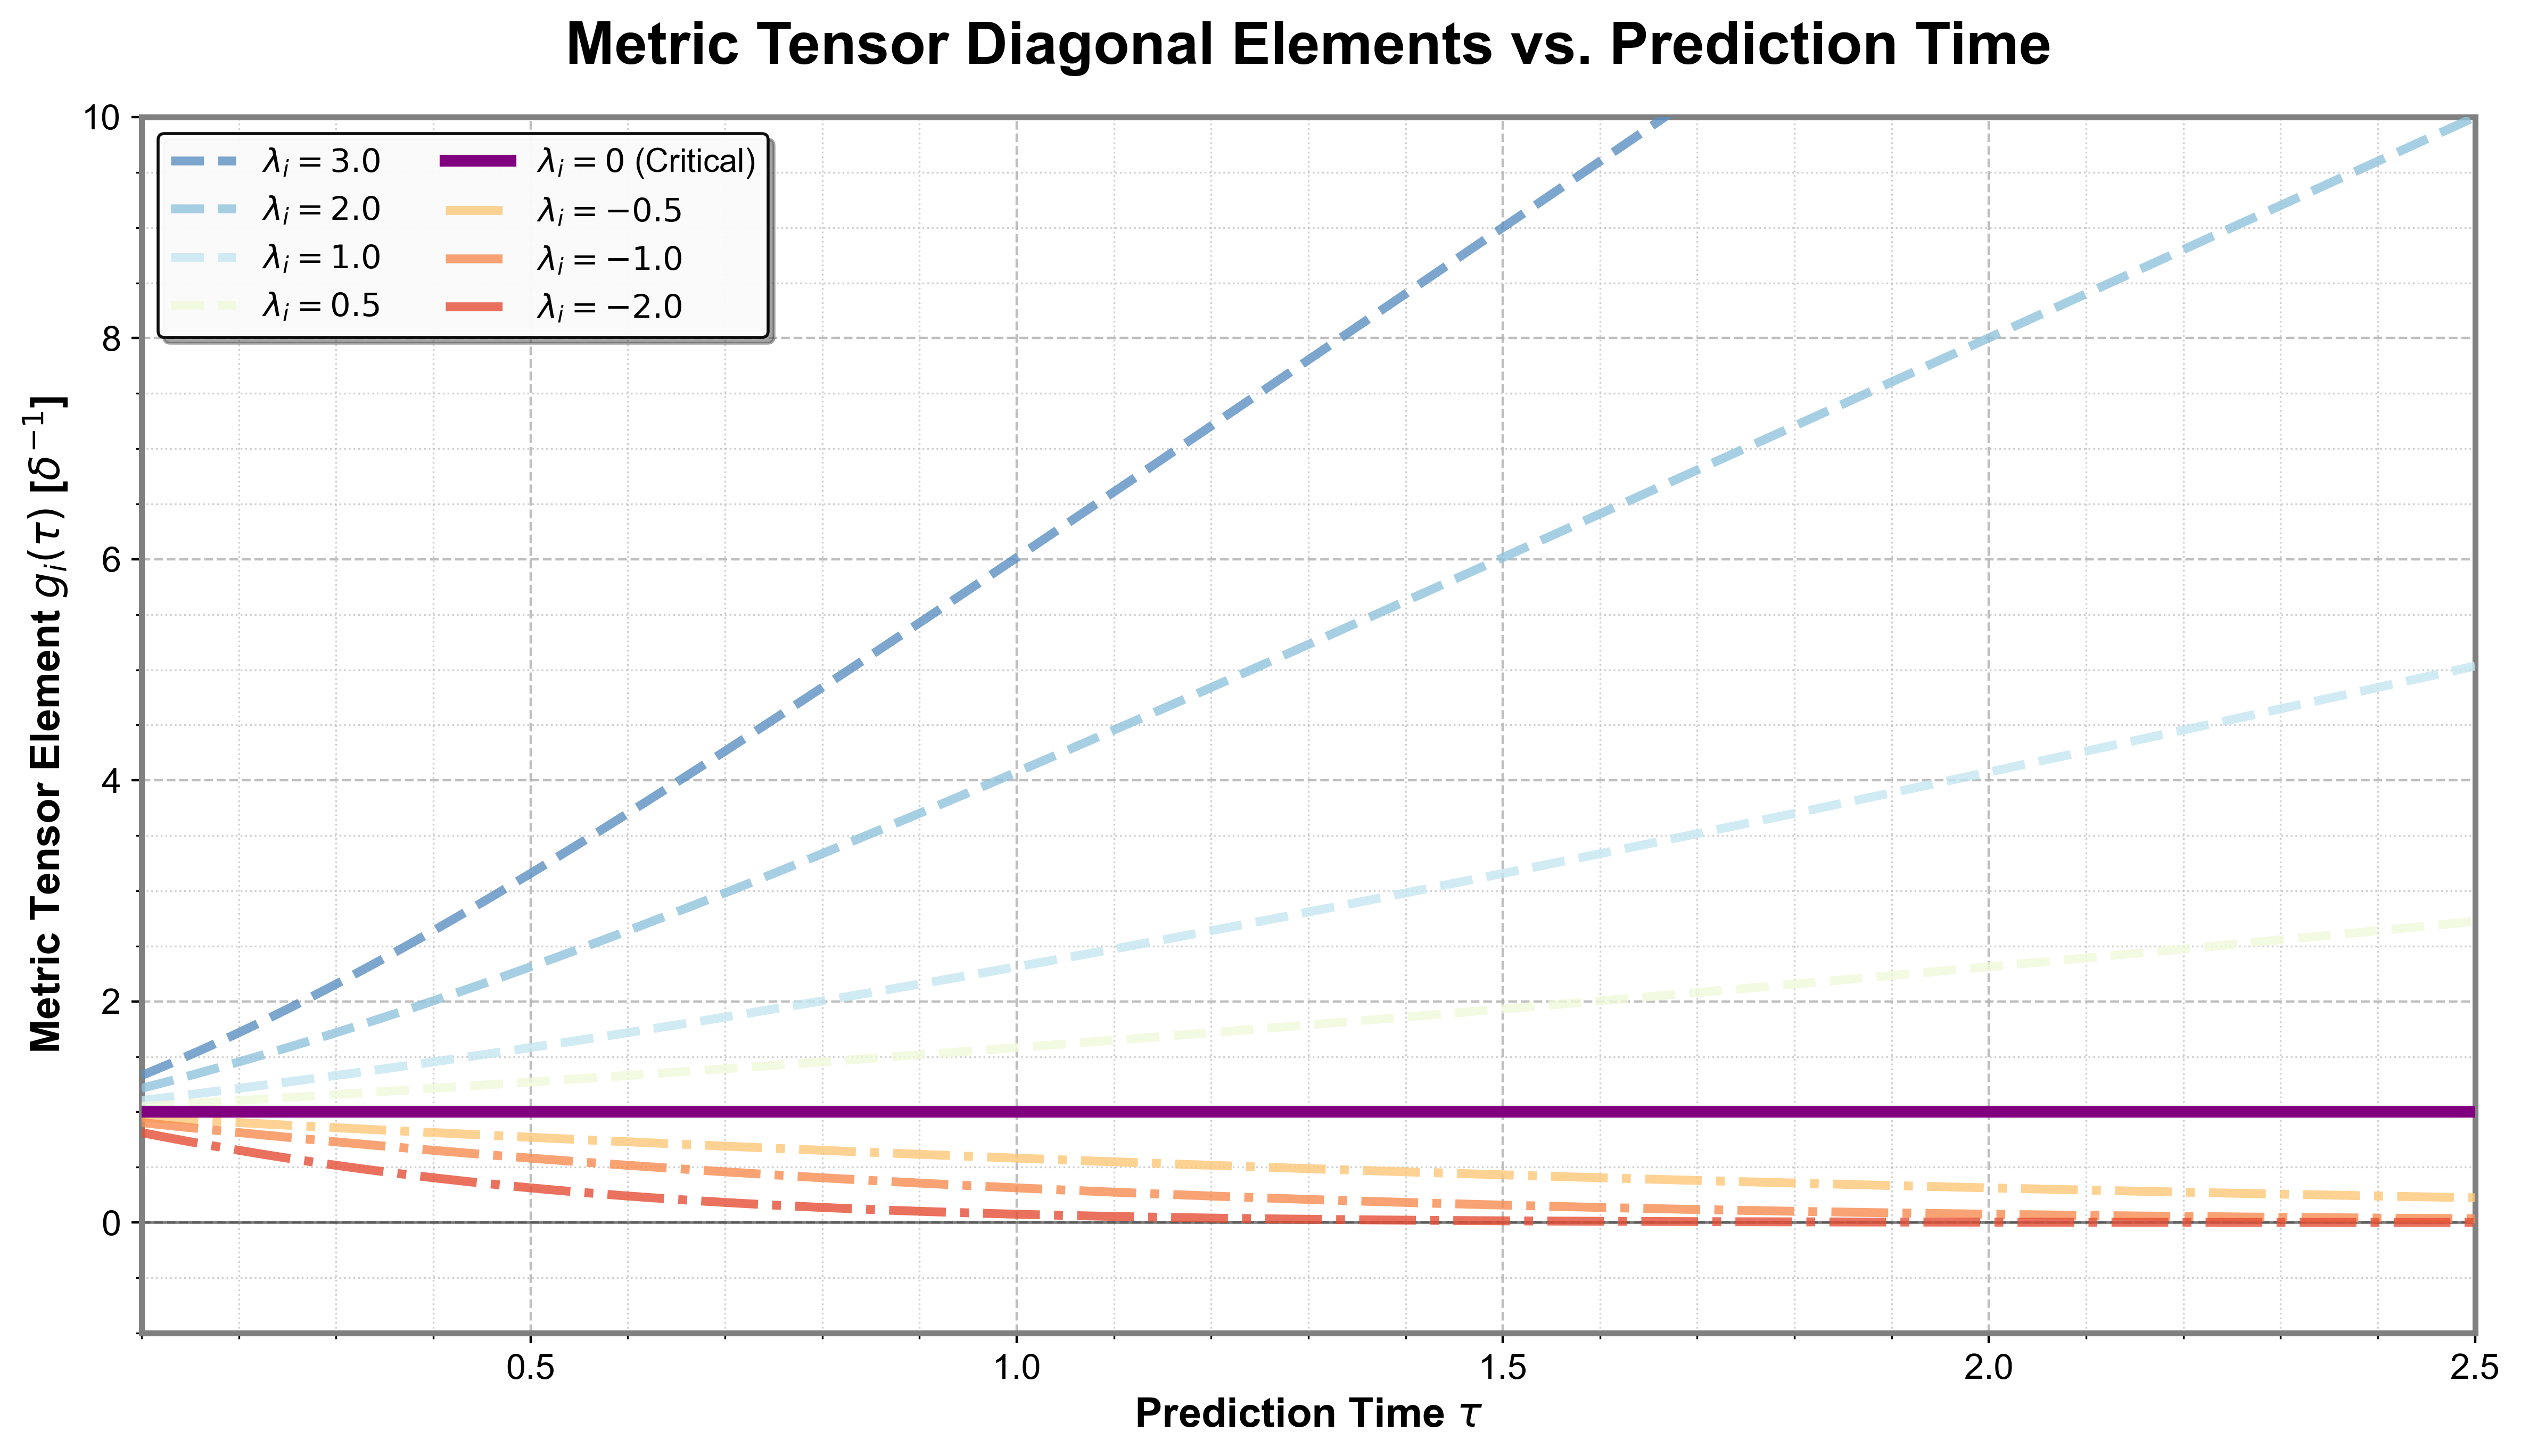
\includegraphics[width=1.00\textwidth]{./assets/metric_tensor_elements.png}
    \caption{度量张量对角元素随预报时间的演化规律。紫色粗线对应中性方向 ($\lambda = 0$)，蓝色系对应稳定方向 ($\lambda < 0$)，红色系对应不稳定方向 ($\lambda > 0$)。}
    \label{fig:metric_vs_tau}
\end{figure}

\textbf{1. 中性方向 ($\eigenval_i = 0$): 准守恒模态}

当 $\eigenval_i = 0$ 时，对应于动力学系统的\textbf{中性方向}，初始扰动既不增长也不衰减。
利用L'Hôpita 法则:
\begin{equation}
\label{eq:metric_neutral}
    [\metric_{\predtime}]_{ii} = \lim_{\eigenval_i \to 0} \frac{2 \eigenval_i \predtime}{\delta_i} \cdot \frac{e^{2 \eigenval_i \predtime}}{e^{2 \eigenval_i \predtime} - 1} = \frac{1}{\delta_i}
\end{equation}

\begin{figure}[htbp]
    \centering
    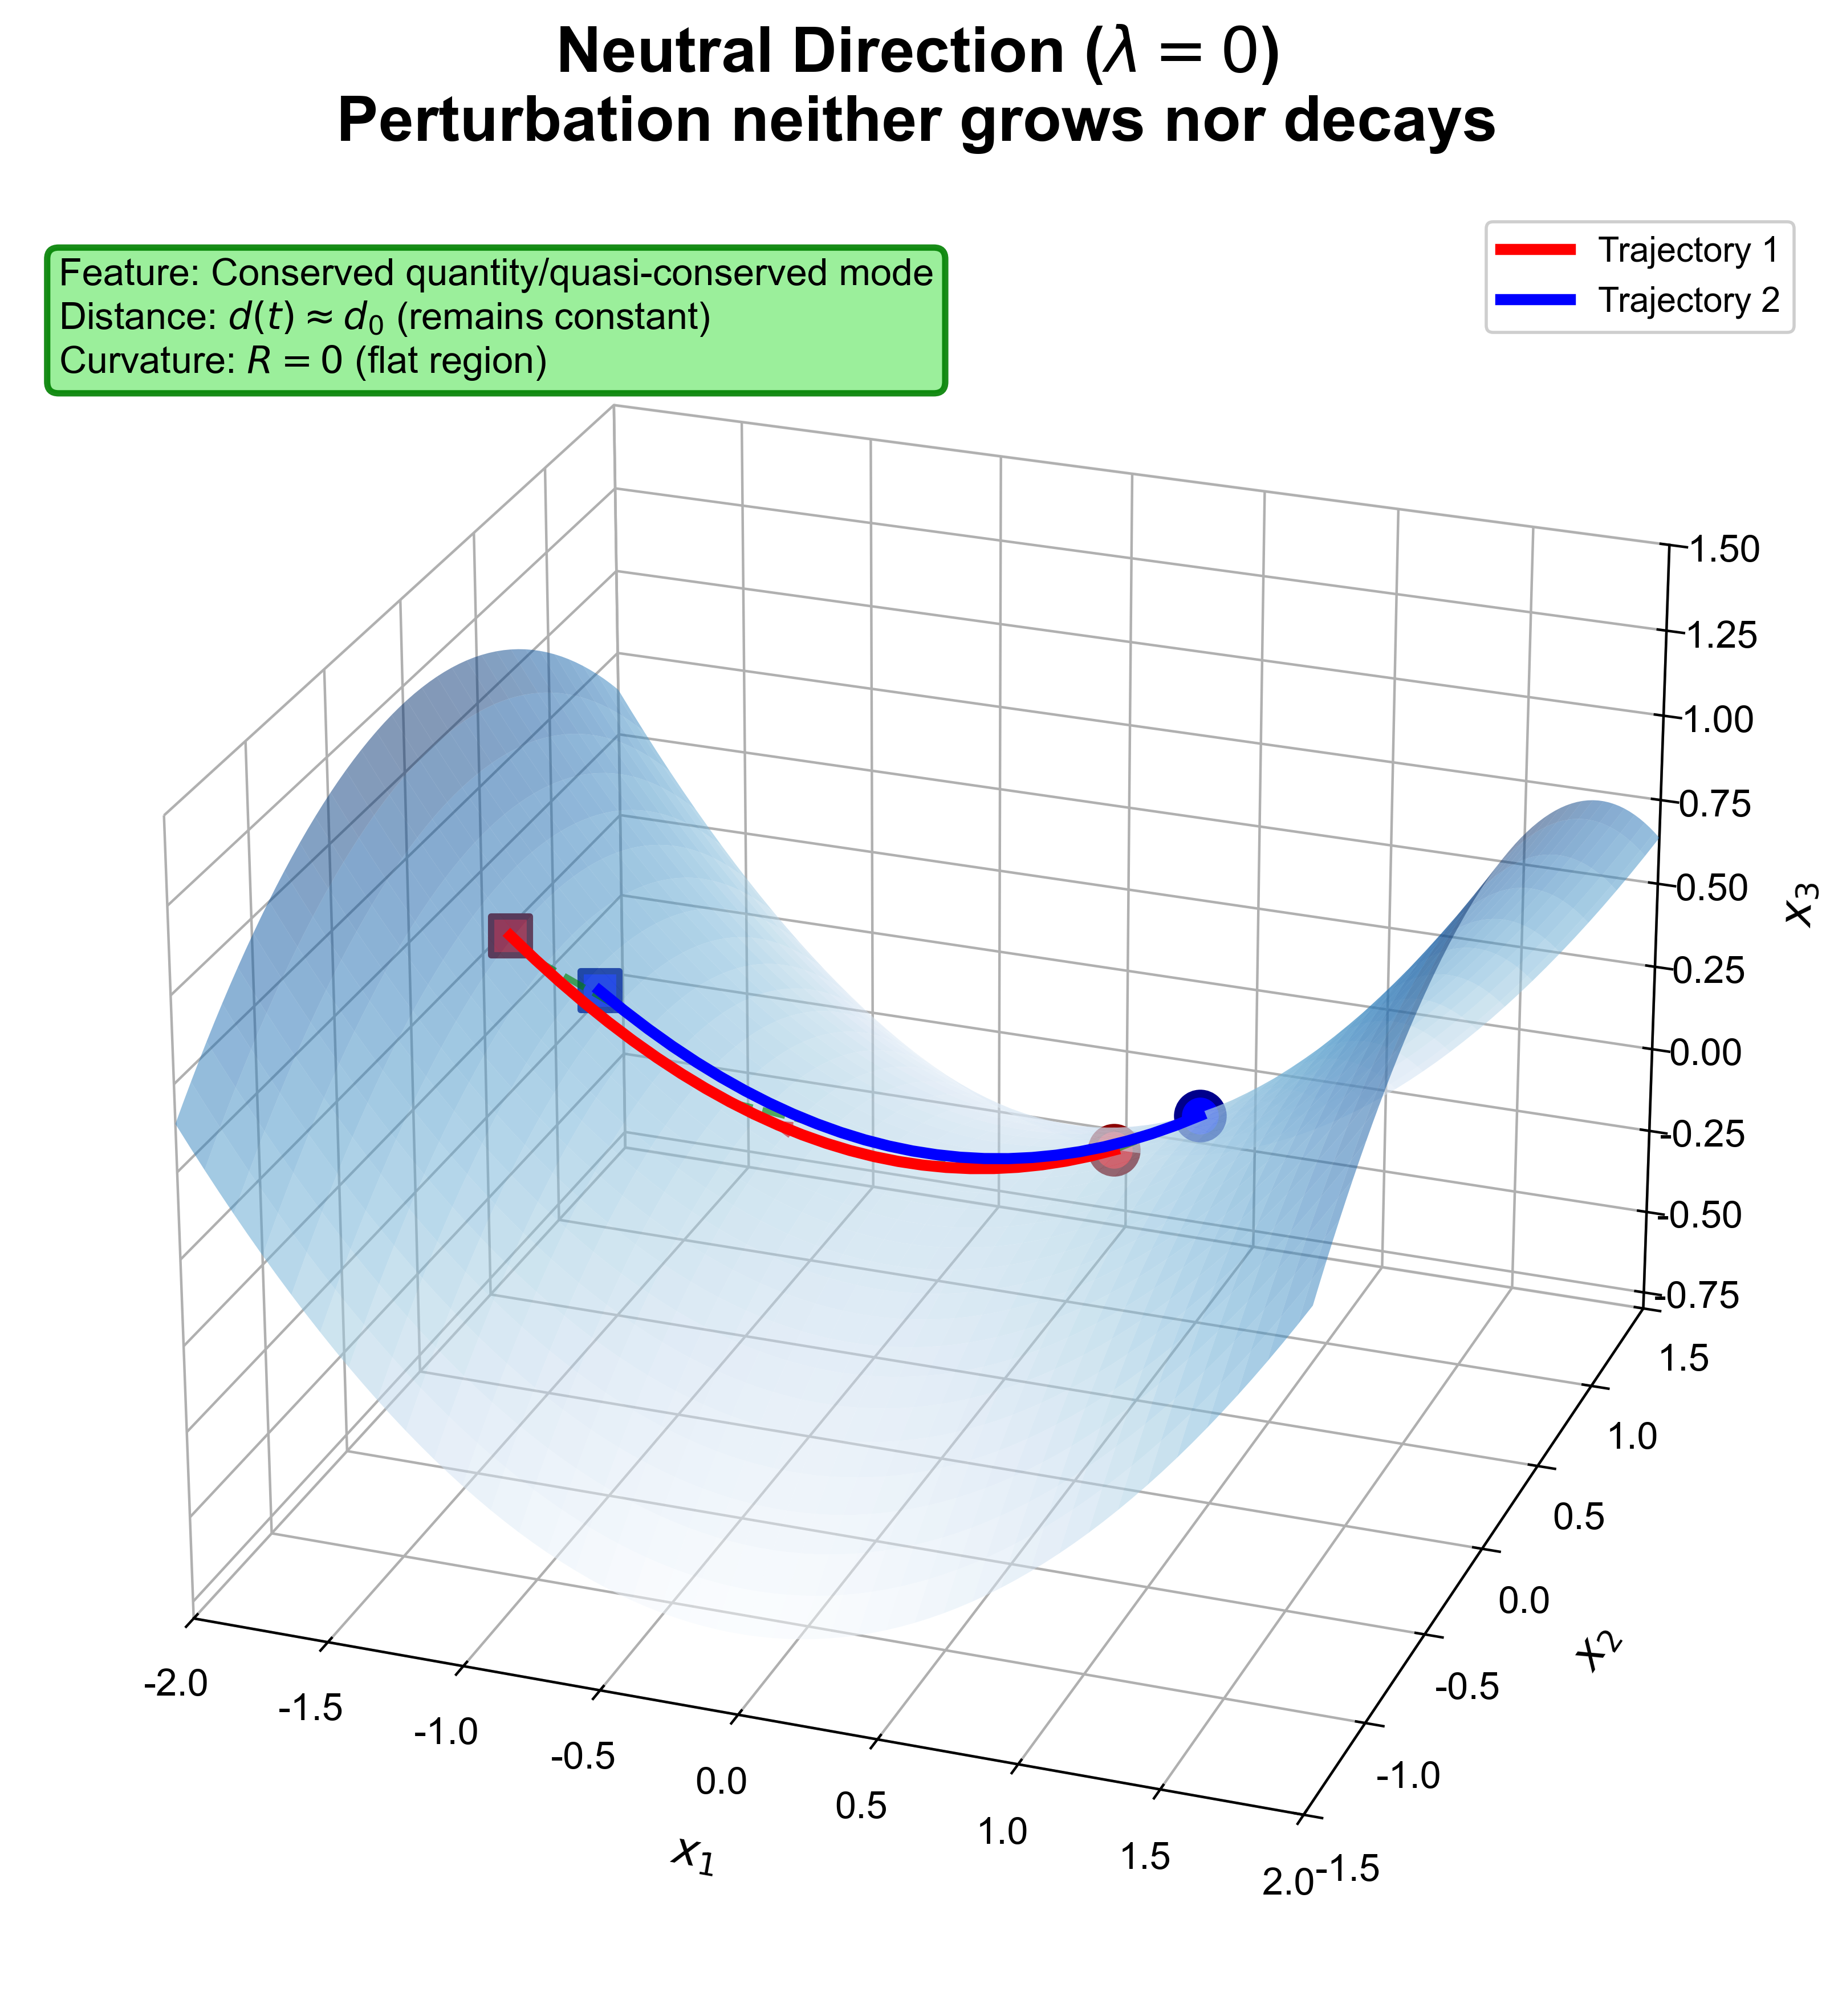
\includegraphics[width=0.56\textwidth]{./assets/neutral_direction.png}
    \caption{中性方向的几何图景。两条轨迹 (红色和蓝色) 从接近的初值出发，沿中性方向演化，距离保持恒定。绿色虚线标示不同时刻的距离。}
    \label{fig:neutral_direction}
\end{figure}

如图 \ref{fig:metric_vs_tau} 和 \ref{fig:neutral_direction} 所示，中性方向的度量保持常数，与预报时间 $\predtime$ 无关。
曲率在该方向上为零，对应流形上的“平坦区域”。
不存在混沌效应的作用，动力学距离完全由扩散控制: $d_{\predtime} \sim \sqrt{1 / \delta_i}$。
时间权重 $\sqrt{\predtime}$ 恰好抵消了扩散导致的 $1/\sqrt{\predtime}$ 衰减。

物理上，中性方向对应\textbf{准守恒模态}，如地转平衡态中的位涡守恒、绝热过程中的熵守恒、海洋盐度-温度补偿关系等。
这些模态的可预报性可以保持较长时间，是季节至年际预报的重要基础 \cite{majda2012climate}。

\textbf{2. 稳定方向 ($\eigenval_i < 0$): 吸引子}

当 $\eigenval_i < 0$ 时，对应于\textbf{稳定方向}。
设 $\eigenval_i = -\mu_i$，其中 $\mu_i > 0$，度量对角元为:
\begin{equation}
\label{eq:metric_stable}
    [\metric_{\predtime}]_{ii} = \frac{2 \mu_i \predtime}{\delta_i} \frac{e^{-2 \mu_i \predtime}}{1 - e^{-2 \mu_i \predtime}} \xrightarrow{\predtime \to \infty} 0
\end{equation}

\begin{figure}[htbp]
    \centering
    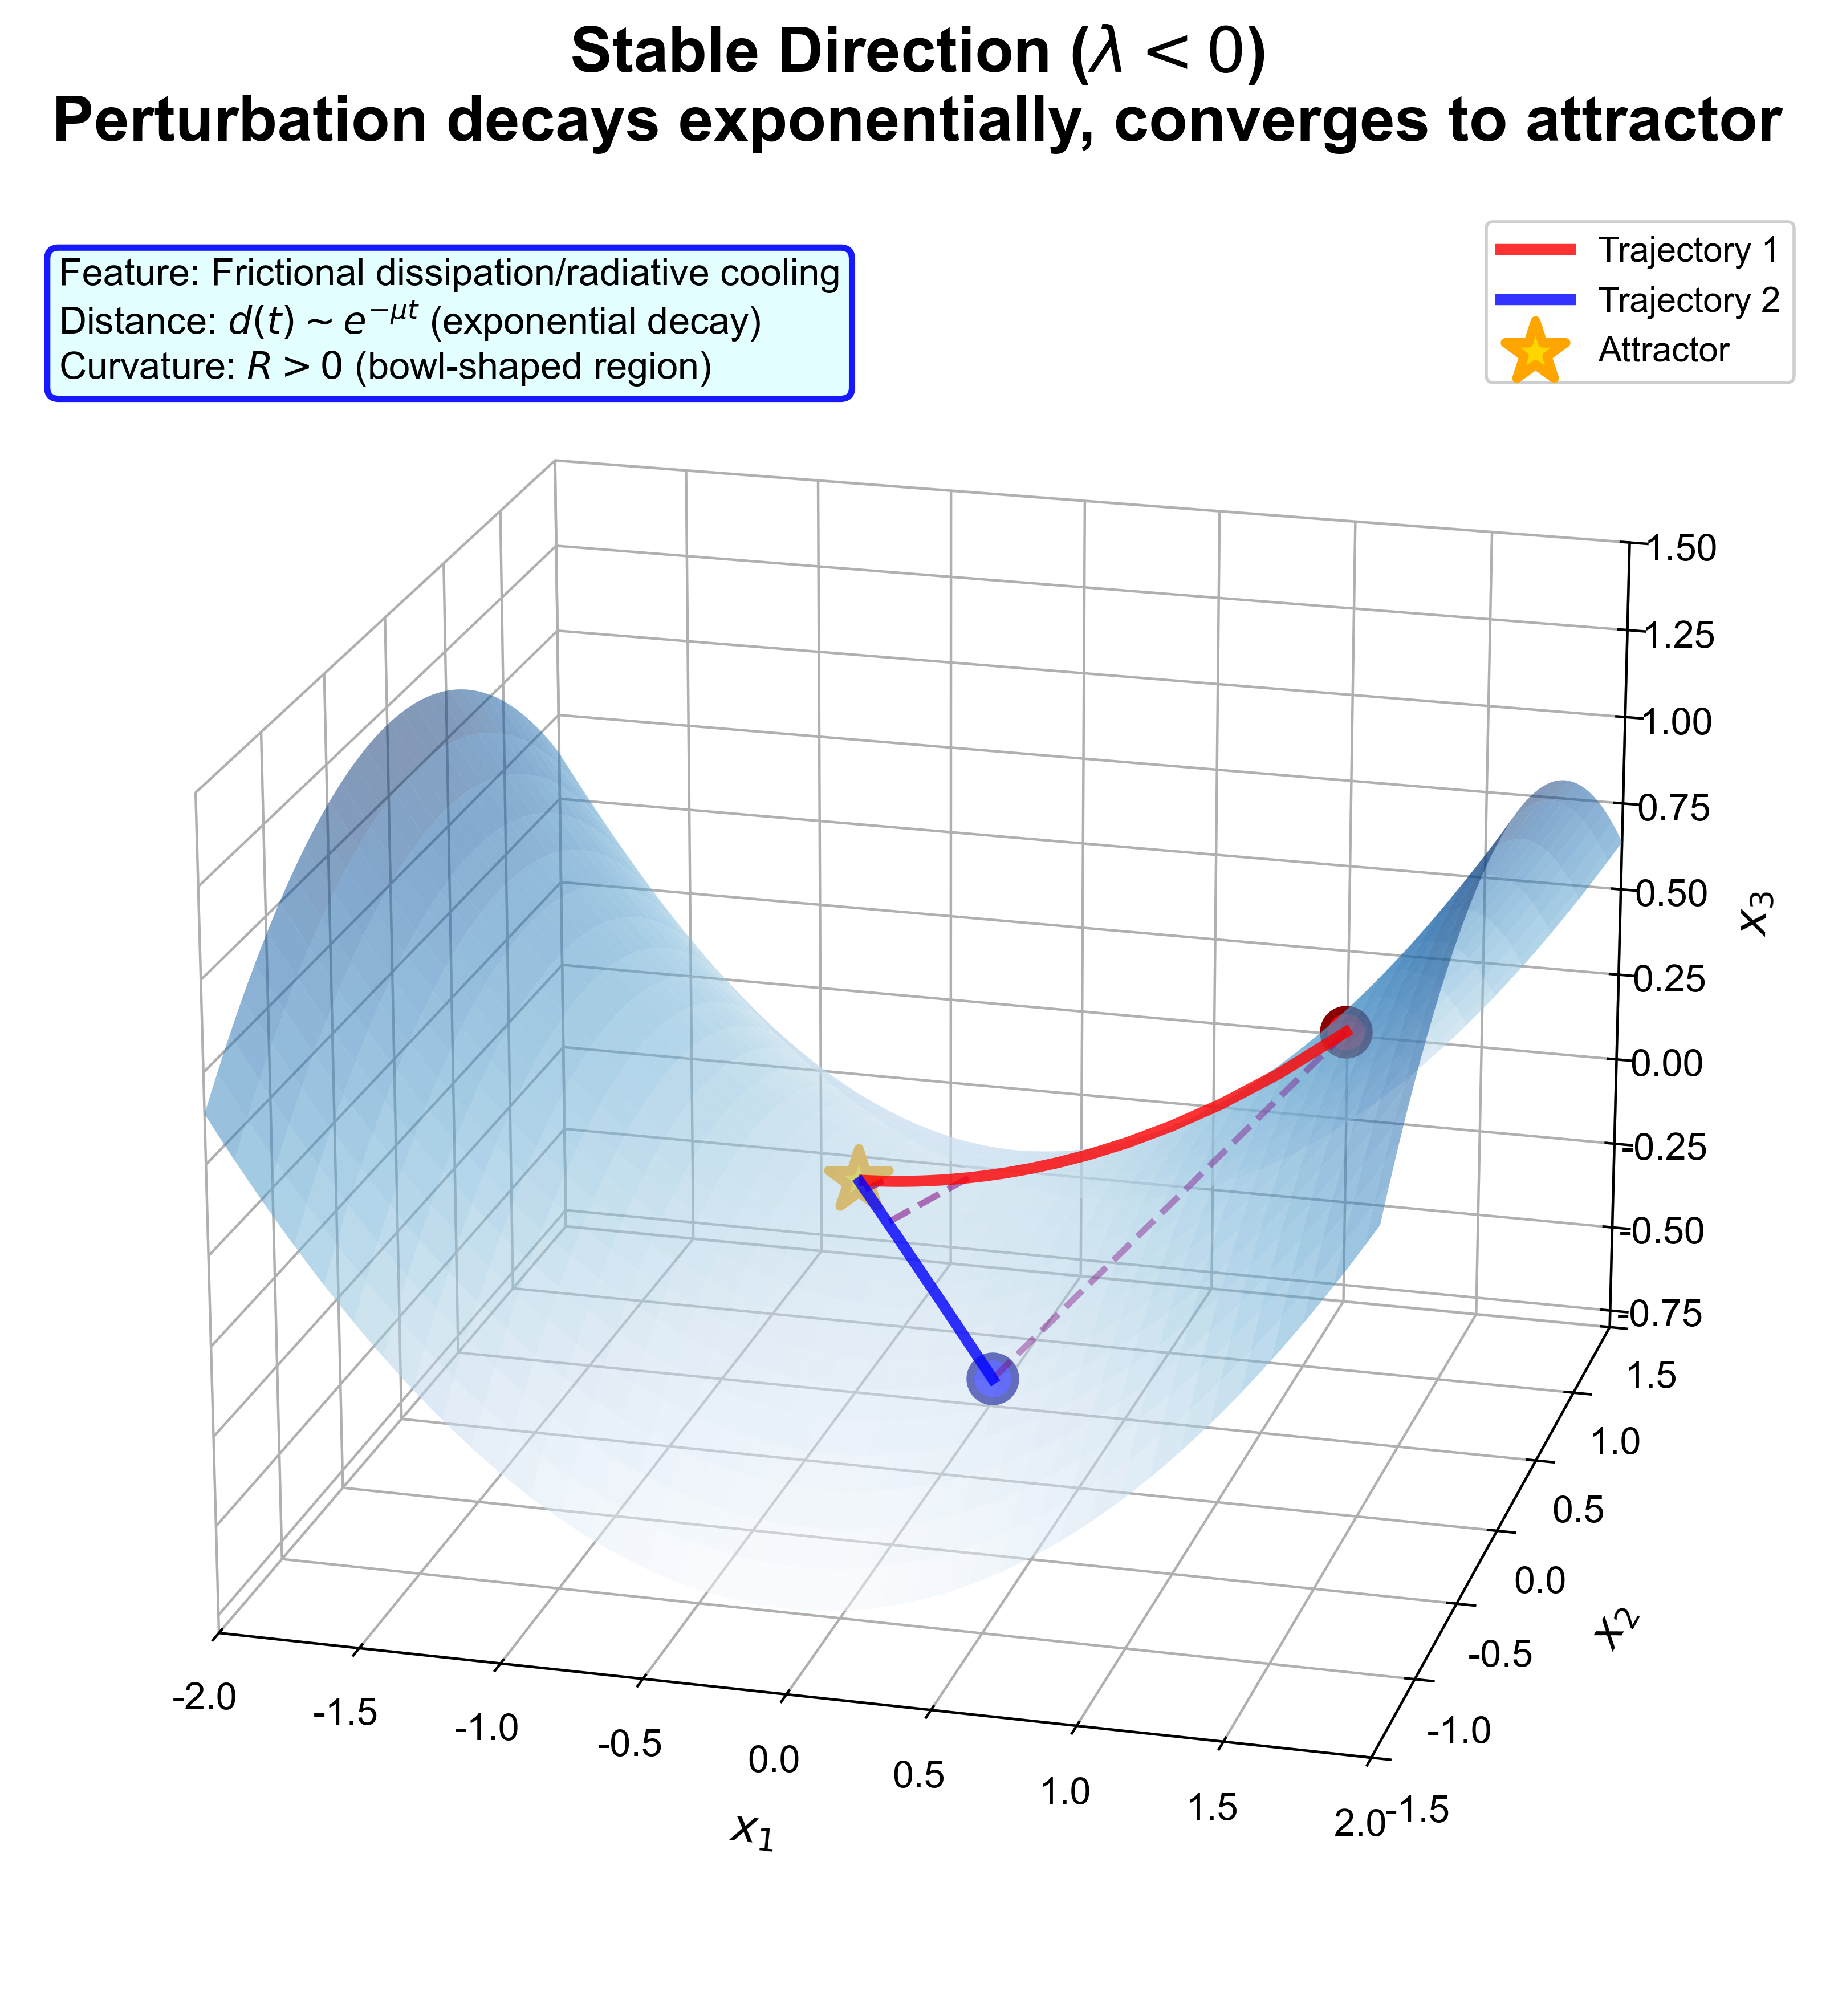
\includegraphics[width=0.56\textwidth]{./assets/stable_direction.png}
    \caption{稳定方向的几何图景。两条轨迹从不同初值出发，沿稳定方向演化，指数收敛到同一吸引子 (金色五角星)。紫色虚线标示距离随时间指数衰减。}
    \label{fig:stable_direction}
\end{figure}

如图 \ref{fig:metric_vs_tau} 和 \ref{fig:stable_direction} 所示，稳定方向的度量呈指数下降，直至趋于零。
曲率为正，对应流形上的“碗状”区域。
沿稳定方向的初始扰动以指数速率 $\mu_i$ 衰减，两条初始接近的轨迹迅速收敛至同一\textbf{吸引子 (Attractor)}。
该方向上的不确定性对未来状态的影响逐渐消失，被吸引子的收缩性抵消。

物理上，稳定方向对应大气中的摩擦耗散、辐射冷却、海洋中的深层混合等过程 \cite{palmer1993extended}。
例如，边界层湍流摩擦导致近地风速扰动快速衰减 ($\meanval \sim 1\,\text{day}^{-1}$)。
吸引子的存在保证了气候系统的\textbf{韧性 (Resilience)}: 即使遭受一定程度的外部冲击，地球系统最终仍将恢复到吸引子上。

\textbf{3. 不稳定方向 ($\eigenval_i > 0$): 混沌效应}

当 $\eigenval_i > 0$ 时，对应于\textbf{不稳定方向}。
雅可比矩阵 $\jacobian_{\drift}$ 的正特征值表征初始扰动的指数增长率 (即Lyapunov指数)，是\textbf{混沌效应 (Chaos Effect)}的动力学根源。

度量对角元为:
\begin{equation}
\label{eq:metric_unstable}
    [\metric_{\predtime}]_{ii} = \frac{2 \eigenval_i \predtime}{\delta_i} \frac{e^{2 \eigenval_i \predtime}}{e^{2 \eigenval_i \predtime} - 1} \xrightarrow{\predtime \to \infty} \frac{2\eigenval_i \predtime}{\delta_i}
\end{equation}

\begin{figure}[htbp]
    \centering
    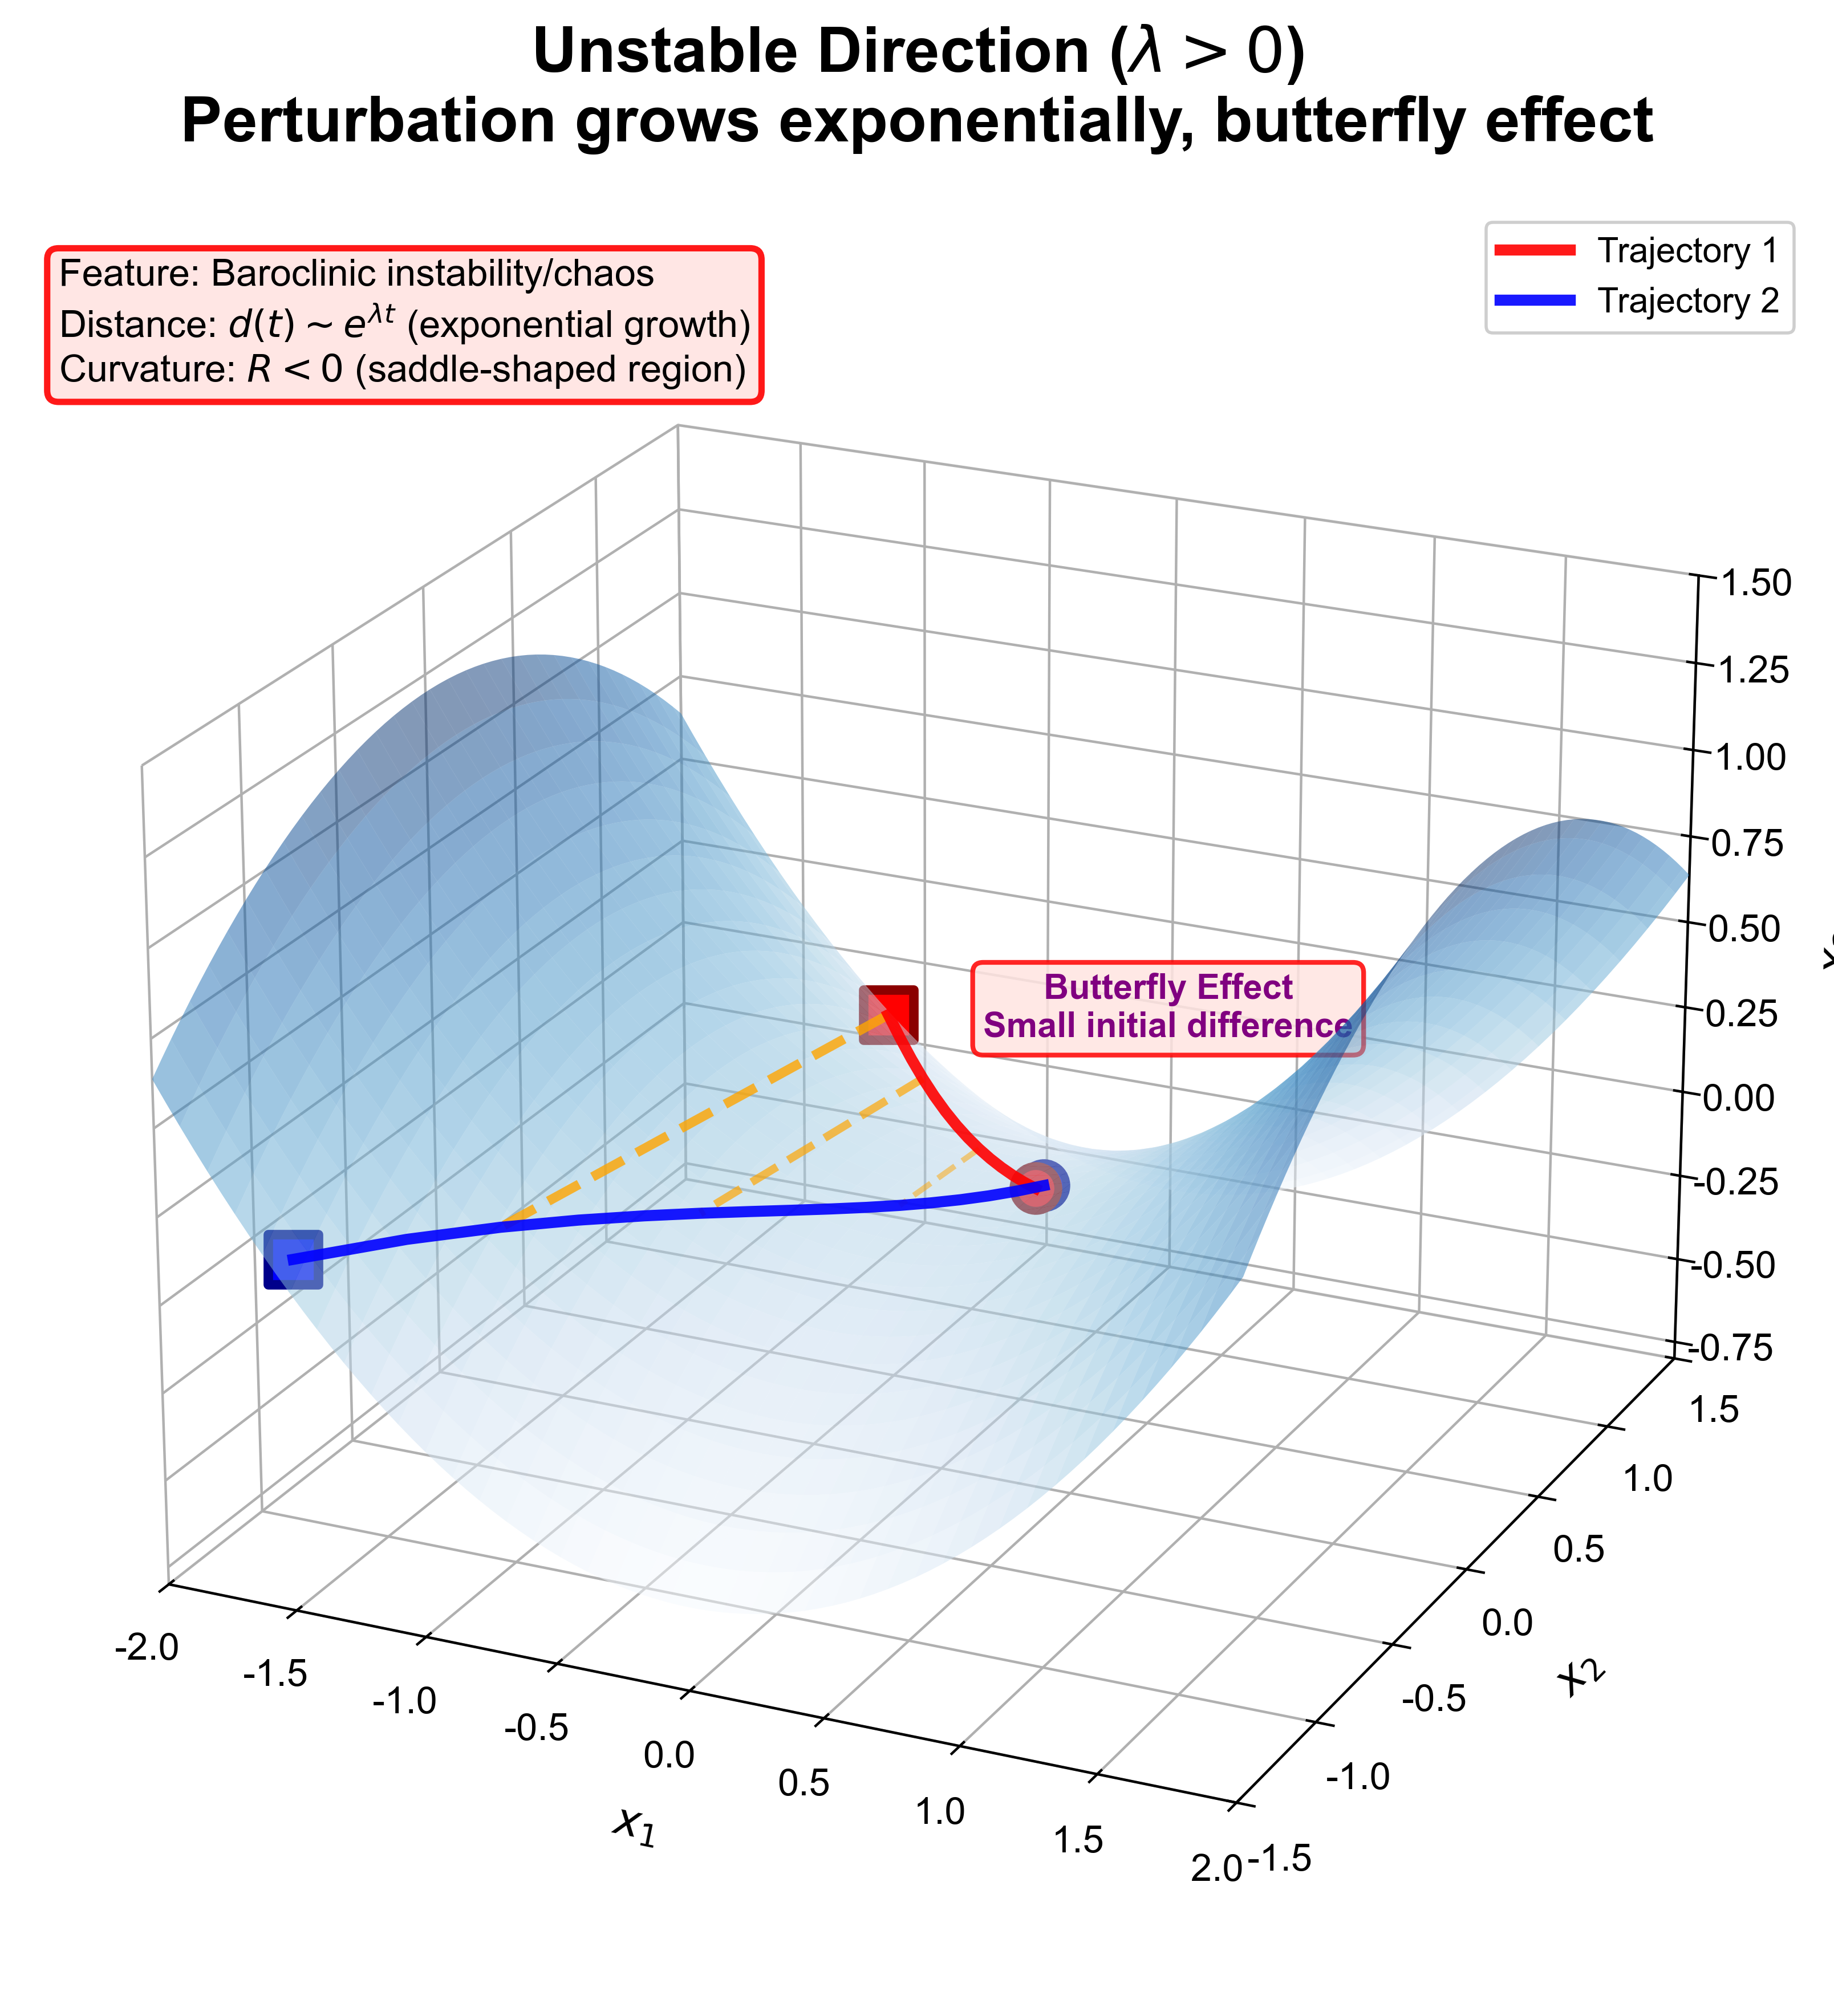
\includegraphics[width=0.56\textwidth]{./assets/unstable_direction.png}
    \caption{不稳定方向的几何图景 (蝴蝶效应)。两条轨迹从极其接近的初值出发 (红色和蓝色点几乎重合)，沿不稳定方向演化，距离指数发散。橙色虚线标示距离随时间指数增长。}
    \label{fig:unstable_direction}
\end{figure}

如图 \ref{fig:metric_vs_tau} 和 \ref{fig:unstable_direction} 所示，不稳定方向的度量呈线性增长趋势。
比例系数 $2\eigenval_i / \delta_i$ 为内禀的可预报性因子，量化了动力学混沌效应与随机噪声扩散的竞争。
曲率在该方向上为负，且绝对值将随着预报时间 $\predtime$ 的增大而线性增大，像是流形上一片正在被不断扭曲的“鞍形区域”。
这是对Lorenz \cite{lorenz1963deterministic} 提出的“蝴蝶效应”的微分几何表述。
系统的可预报性将随着预报时间的拉长而迅速降低，成为预报技巧损失的主导因素。

物理上，不稳定方向对应大气动力学中的正压不稳定和斜压不稳定模态。
初始扰动沿此方向呈指数增长，表现为天气尺度扰动的快速发展 (如锋生、气旋加深) \cite{palmer1993extended}。

\newpage

\section{基于扩散模型的流形学习}
\label{sec:deep_learning}

一个关键的问题是: 如何在数值上解析流形的几何结构和随机动力学算子？
我们面临着许多困难: 流形 $\manifold$ 的维度与嵌入模式未知；动力学算子 $\drift, \difftensor$ 没有解析表达式，基于第一性原理的建模又过于复杂；度量张量 $\metric$ 依赖于过多较强的简化假设，且显式计算需要求高阶导数 $\jacobian_{\drift}$，这在高维系统中是不可行的。

幸运的是，长期以来我们已经积累了海量的历史观测资料。
数据驱动的方法因此成为了可能——我们可以直接从数据中学习流形，而无需描述复杂的物理建过程。
\textbf{扩散模型 (Diffusion Models)} 为此提供了理想的工具，其通过评分函数 $\nabla_{\fastvar} \log p(\fastvar)$ 隐式表示了流形的概率几何。
本章将结合前述数学框架，介绍扩散模型是如何从观测中重构流形 $\manifold$ 与演化算子 $\evolop_t$ 的。

\subsection{扩散模型}

扩散模型的核心思想源于非平衡统计力学: 设计一个可控的扩散过程，将复杂的数据分布 $p_{\text{data}}(\fastvar)$ 逐步映射为简单的先验分布 (通常为标准高斯 $\normdist(0, I)$)，再通过学习逆向过程从先验噪声中重构数据。
定义正向扩散为Ornstein-Uhlenbeck过程:
\begin{equation}
\label{eq:forward_diffusion}
    d\fastvar_t = -\frac{1}{2}\beta(t)\fastvar_t\,dt + \sqrt{\beta(t)}\,d\wiener_t, \quad t \in [0, T]
\end{equation}

其中 $\beta(t) > 0$ 为噪声调度函数，$\wiener_t$ 是标准布朗运动。
该过程的解析解为 $\fastvar_t = \sqrt{\bar{\alpha}_t}\,\fastvar_0 + \sqrt{1-\bar{\alpha}_t}\,\bm{\epsilon}$，其中 $\bm{\epsilon} \sim \normdist(0, I)$ 且 $\bar{\alpha}_t = \exp(-\frac{1}{2}\int_0^t \beta(s)\,ds)$。
当 $t \to T$ 且 $\bar{\alpha}_T \to 0$ 时，$\fastvar_T$ 的边缘分布收敛至 $\normdist(0, I)$，数据的结构信息被噪声完全淹没。

逆向过程的关键在于Anderson定理 \cite{anderson1982reverse}: 正向扩散SDE在时间反转下仍为SDE，其漂移项由评分函数决定:
\begin{equation}
\label{eq:reverse_diffusion}
    d\fastvar_t = \left[\frac{1}{2}\beta(t)\fastvar_t - \beta(t)\nabla_{\fastvar} \log p_t(\fastvar_t)\right]dt + \sqrt{\beta(t)}\,d\bar{\wiener}_t
\end{equation}

这里 $\bar{\wiener}_t$ 是反向时间的布朗运动，$\nabla_{\fastvar} \log p_t$ 称为时刻 $t$ 的评分函数。
若能准确估计评分函数，则从 $\fastvar_T \sim \normdist(0, I)$ 出发，沿方程 \eqref{eq:reverse_diffusion} 积分至 $t=0$，即可采样得到 $\fastvar_0 \sim p_{\text{data}}$。
这一逆向过程可理解为沿概率密度梯度的引导扩散: 在每个时刻，系统既受随机扰动 (布朗运动项)，又受评分函数的漂移驱动，后者将样本推向高概率密度区域，最终收敛至数据流形。

我们通过\textbf{去噪评分匹配 (Denoising Score Matching)} 实现对评分函数的估计 \cite{vincent2011connection}。
考虑到 $p(\fastvar_t|\fastvar_0) = \normdist(\sqrt{\bar{\alpha}_t}\fastvar_0, (1-\bar{\alpha}_t)I)$，其评分为 $\nabla_{\fastvar_t} \log p(\fastvar_t|\fastvar_0) = -\frac{\fastvar_t - \sqrt{\bar{\alpha}_t}\fastvar_0}{1-\bar{\alpha}_t} = -\frac{\bm{\epsilon}}{\sqrt{1-\bar{\alpha}_t}}$。
因此，训练神经网络 $\bm{\epsilon}_\theta(\fastvar_t, t)$ 预测噪声 $\bm{\epsilon}$，等价于学习评分函数:
\begin{equation}
\label{eq:denoising_loss}
    \mathcal{L}_{\text{denoise}} = \E_{t \sim \mathcal{U}[0,T], \fastvar_0 \sim p_{\text{data}}, \bm{\epsilon} \sim \normdist(0,I)}\left[\left\|\bm{\epsilon}_\theta\left(\sqrt{\bar{\alpha}_t}\fastvar_0 + \sqrt{1-\bar{\alpha}_t}\bm{\epsilon}, t\right) - \bm{\epsilon}\right\|^2\right]
\end{equation}

这一目标函数将评分匹配转化为标准的监督学习问题: 对于每个训练样本 $\fastvar_0$，随机采样噪声水平 $t$ 和高斯噪声 $\bm{\epsilon}$，构造加噪样本 $\fastvar_t$，训练网络从 $\fastvar_t$ 重构 $\bm{\epsilon}$。
训练完成后，神经网络 $\bm{\epsilon}_\theta$ 隐式地参数化了全时间区间 $[0,T]$ 上评分函数族 $\{\nabla \log p_t\}_{t \in [0,T]}$。

\subsection{流形的隐式表示}

扩散模型学习流形的机制可从评分函数的几何意义理解。
回顾流形假设 (假设 \ref{ass:manifold_hypothesis}): 数据分布 $p_{\text{data}}$ 的支撑集为低维流形 $\manifold \subset \dataspace$，$\dim(\manifold) = \manifolddim \ll N$。
在流形外，概率密度 $p_{\text{data}}(\fastvar) = 0$；在流形内部及其邻域，密度函数沿流形的法空间快速衰减。
因此，评分函数 $\nabla \log p_{\text{data}}$ 在流形上指向密度梯度方向，其分量可分解为切向分量 (沿流形内的密度变化) 和法向分量 (指向流形方向)。
当样本偏离流形时，法向分量占主导，评分函数强烈地将其拉回流形；当样本位于流形内部时，切向分量引导其沿流形表面向高密度区域移动。

在扩散模型的正向过程中，噪声的注入使得中间分布 $p_t$ 的支撑集从低维流形 $\manifold$ 扩展至全空间 $\dataspace$，但流形的几何结构以软约束的形式保留在 $p_t$ 的统计特征中。
逆向过程则沿评分函数的梯度流逐步收缩分布支撑: 从全空间的高斯分布出发，评分函数引导样本穿越概率场景，最终收敛至低维流形。
这一过程可视为\textbf{几何退火 (Geometric Annealing)}: 高噪声水平 ($t$ 接近 $T$) 时，评分函数捕获全局拓扑结构；低噪声水平 ($t$ 接近 $0$) 时，评分函数细化局部流形几何。
多尺度的去噪过程隐式地学习了流形的层次表示。

另外，我们考虑评分函数的Hessian矩阵 $\nabla^2 \log p_{\text{data}}$，即\textbf{Fisher信息矩阵}。
在统计流形理论中，Fisher信息矩阵定义了参数空间的黎曼度量，量化了概率分布对参数扰动的敏感性。
在数据流形上，$\nabla^2 \log p_{\text{data}}$ 的特征值分解揭示了流形的主曲率方向: 沿流形切空间的特征值反映了密度函数的内在变化率，而沿法空间的特征值则表征了分布从流形向环境空间的衰减速度。
扩散模型通过学习评分函数，隐式地近似了流形的几何结构，使得逆向采样自然地适应流形的局部曲率与全局拓扑。

\subsection{条件生成框架}

将扩散模型扩展至条件生成框架，可实现对地球系统未来状态的概率预报。
设 $\fastvar_0$ 为初始状态，$\fastvar_{\predtime}$ 为时间 $\predtime$ 后的未来状态，目标是学习条件分布 $p(\fastvar_{\predtime}|\fastvar_0)$。
在条件扩散模型中，将初始条件 $\fastvar_0$ 编码为神经网络的额外输入，修改噪声预测器为 $\bm{\epsilon}_\theta(\fastvar_t, t, \fastvar_0)$，训练目标变为:
\begin{equation}
\label{eq:conditional_diffusion}
    \mathcal{L}_{\text{cond}} = \E_{t, \fastvar_0, \fastvar_{\predtime}, \bm{\epsilon}}\left[\left\|\bm{\epsilon}_\theta\left(\sqrt{\bar{\alpha}_t}\,\fastvar_{\predtime} + \sqrt{1-\bar{\alpha}_t}\,\bm{\epsilon}, t, \fastvar_0\right) - \bm{\epsilon}\right\|^2\right]
\end{equation}

其中期望对 $(\fastvar_0, \fastvar_{\predtime})$ 的联合分布求取，该分布可从历史观测轨迹中采样得到。
训练完成后，推理时从 $\fastvar_T \sim \normdist(0, I)$ 开始，沿条件逆向SDE积分:
\begin{equation}
\label{eq:conditional_reverse}
    d\fastvar_t = \left[\frac{1}{2}\beta(t)\fastvar_t - \beta(t)\nabla_{\fastvar} \log p_t(\fastvar_t|\fastvar_0)\right]dt + \sqrt{\beta(t)}\,d\bar{\wiener}_t
\end{equation}

得到 $\fastvar_{\predtime}$ 的一次采样。
重复采样 $M$ 次，即得集合预报 $\{\fastvar_{\predtime}^{(i)}\}_{i=1}^M$，其经验分布逼近条件概率 $p(\fastvar_{\predtime}|\fastvar_0)$。
相比确定性预报模型，条件扩散模型自然地量化了预测不确定性: 集合成员的分散度反映了动力学演化的内在随机性与初值敏感性。

条件生成框架实际上与第 \ref{sec:sde_measure} 章中的随机动力学过程是一致的。
方程 \eqref{eq:conditional_reverse} 中的条件评分函数 $\nabla \log p_t(\fastvar_t|\fastvar_0)$ 编码了从初值 $\fastvar_0$ 出发的动力学流的几何信息。
在小噪声极限下 ($\beta(t) \to 0$)，逆向SDE退化为确定性ODE，对应于动力学系统的平均场演化；在有限噪声下，扩散项捕获了次网格过程与参数化不确定性的随机效应。
因此，条件扩散模型可视为在概率测度空间 $\mathcal{P}(\manifold)$ 上学习演化算子 $\evolop_t^*: \mathcal{P}(\manifold) \to \mathcal{P}(\manifold)$ 的非参数估计，其中 $\evolop_t^*$ 将初值分布映射为未来时刻的分布。

事实上，条件生成框架还隐式地学习了度量张量。
在扩散模型框架下，记 $\Delta p_t(\fastvar|\fastvar_A, \fastvar_B) := p_t(\fastvar|\fastvar_B) - p_t(\fastvar|\fastvar_A)$ 为两初值条件下时刻 $t$ 的概率密度差。
当 $\|\fastvar_B - \fastvar_A\|$ 充分小时，$\Delta p_t$ 可由评分函数的差分近似:
\begin{equation}
\label{eq:delta_p_score}
    \Delta p_t(\fastvar|\fastvar_A, \fastvar_B) \approx p_t(\fastvar|\fastvar_A) \cdot (\fastvar_B - \fastvar_A)^\top \nabla_{\fastvar_0} \nabla_{\fastvar} \log p_t(\fastvar|\fastvar_A)
\end{equation}

这里 $\nabla_{\fastvar_0} \nabla_{\fastvar} \log p_t$ 是条件评分函数关于初值的梯度，其Frobenius范数的积分量化了初值扰动对整个条件分布的影响:
\begin{equation}
\label{eq:metric_from_score}
    \|\Delta p_t\|_{L^2}^2 \propto (\fastvar_B - \fastvar_A)^\top \underbrace{\int_{\dataspace} p_t(\fastvar|\fastvar_A) \left[\nabla_{\fastvar_0} \nabla_{\fastvar} \log p_t\right]^\top \left[\nabla_{\fastvar_0} \nabla_{\fastvar} \log p_t\right] d\fastvar}_{\text{等效度量张量 } \tilde{\metric}_t} (\fastvar_B - \fastvar_A)
\end{equation}

因此，扩散模型通过学习评分函数，隐式地构造了度量张量。

\newpage

\section{对气候变化的数学建模}
\label{sec:climate_change}

在 \ref{sec:earth_system}、\ref{sec:sde_measure}、\ref{sec:metric_tensor} 章中，我们已经建立了一套描述地球系统的理论框架。
本章将基于该框架，从数学角度重新审视气候变化问题。
我们提出，\textbf{气候变化的本质是由慢变量演化驱动的随机动力系统族的时间依赖过程}。

\subsection{基础定义}

地球系统由快变量 $\fastvar$ 和慢变量 $\slowvar$ 共同描述，其中快变量演化遵循Itô SDE \eqref{eq:sde}，而慢变量在天气时间尺度上近似不变 (假设 \ref{ass:timescale_separation})。
我们可以将气候理解为以慢变量为参数的随机动力系统。

\begin{definition}[气候]
\label{def:climate}
    气候是以慢变量 $\slowvar$ 为参数的随机动力系统:
    \begin{equation}
    \label{eq:climate_system}
        \mathrm{Clim}(\slowvar) = (\manifold_{\slowvar}, \drift_{\slowvar}, \diffop_{\slowvar})
    \end{equation}

    其中 $\manifold_{\slowvar}$ 是由约束定义的低维状态流形，$\drift_{\slowvar}$ 和 $\diffop_{\slowvar}$ 分别是漂移向量场和扩散算子。该动力系统诱导出稳态概率测度 $\measure_{\slowvar}$ (通过 Fokker-Planck 方程 \eqref{eq:steady_fp}) 和黎曼度量 $\metric_{\slowvar}$ (通过方程 \eqref{eq:metric_tensor_final})。
\end{definition}

与气候相对应的是天气，后者指的是系统在相空间中的具体演化轨迹。

\begin{definition}[天气]
\label{def:weather}
    天气是快变量 $\fastvar$ 在流形 $\manifold_{\slowvar}$ 上的一次随机轨迹 $\{\fastvar_t\}_{t \in [0, T]}$，即按照Itô SDE \eqref{eq:sde} 采样得到的一条路径。
\end{definition}

当慢变量 $\slowvar(t)$ (如温室气体浓度、太阳辐射、冰盖体积等) 随时间演化时，随机动力系统随之发生改变，这一过程即为气候变化，数学上可以表述为:
\begin{equation}
\label{eq:climate_change_evolution}
    \mathrm{Clim}(\slowvar(t)) = (\manifold_{\slowvar(t)}, \drift_{\slowvar(t)}, \diffop_{\slowvar(t)}), \quad t \in [t_0, t_1]
\end{equation}

为了刻画气候系统的长期行为，我们引入吸引子的概念。
吸引子是系统在长时间演化后趋向的集合，我们通过概率测度的支撑集给出其定义。

\begin{definition}[吸引子]
\label{def:attractor}
    设随机动力学过程在流形 $\manifold_{\slowvar}$ 上演化。集合 $\attractor_{\slowvar} \subset \manifold_{\slowvar}$ 称为吸引子，若其是概率测度 $\measure_{\slowvar}$ 的支撑集:
    \begin{equation}
    \label{eq:attractor_def}
        \attractor_{\slowvar} = \mathrm{supp}(\measure_{\slowvar})
    \end{equation}

    即 $\measure_{\slowvar}(\attractor_{\slowvar}) = 1$ 且 $\attractor_{\slowvar}$ 是满足此条件的最小闭集。
\end{definition}

吸引子的拓扑结构刻画了气候系统的相结构 (Phase Structure)。
根据慢变量演化过程中吸引子的拓扑结构是否改变，我们可以将气候变化分为两类，如图 \ref{fig:climate_change_types} 所示。

\begin{figure}[htbp]
    \centering
    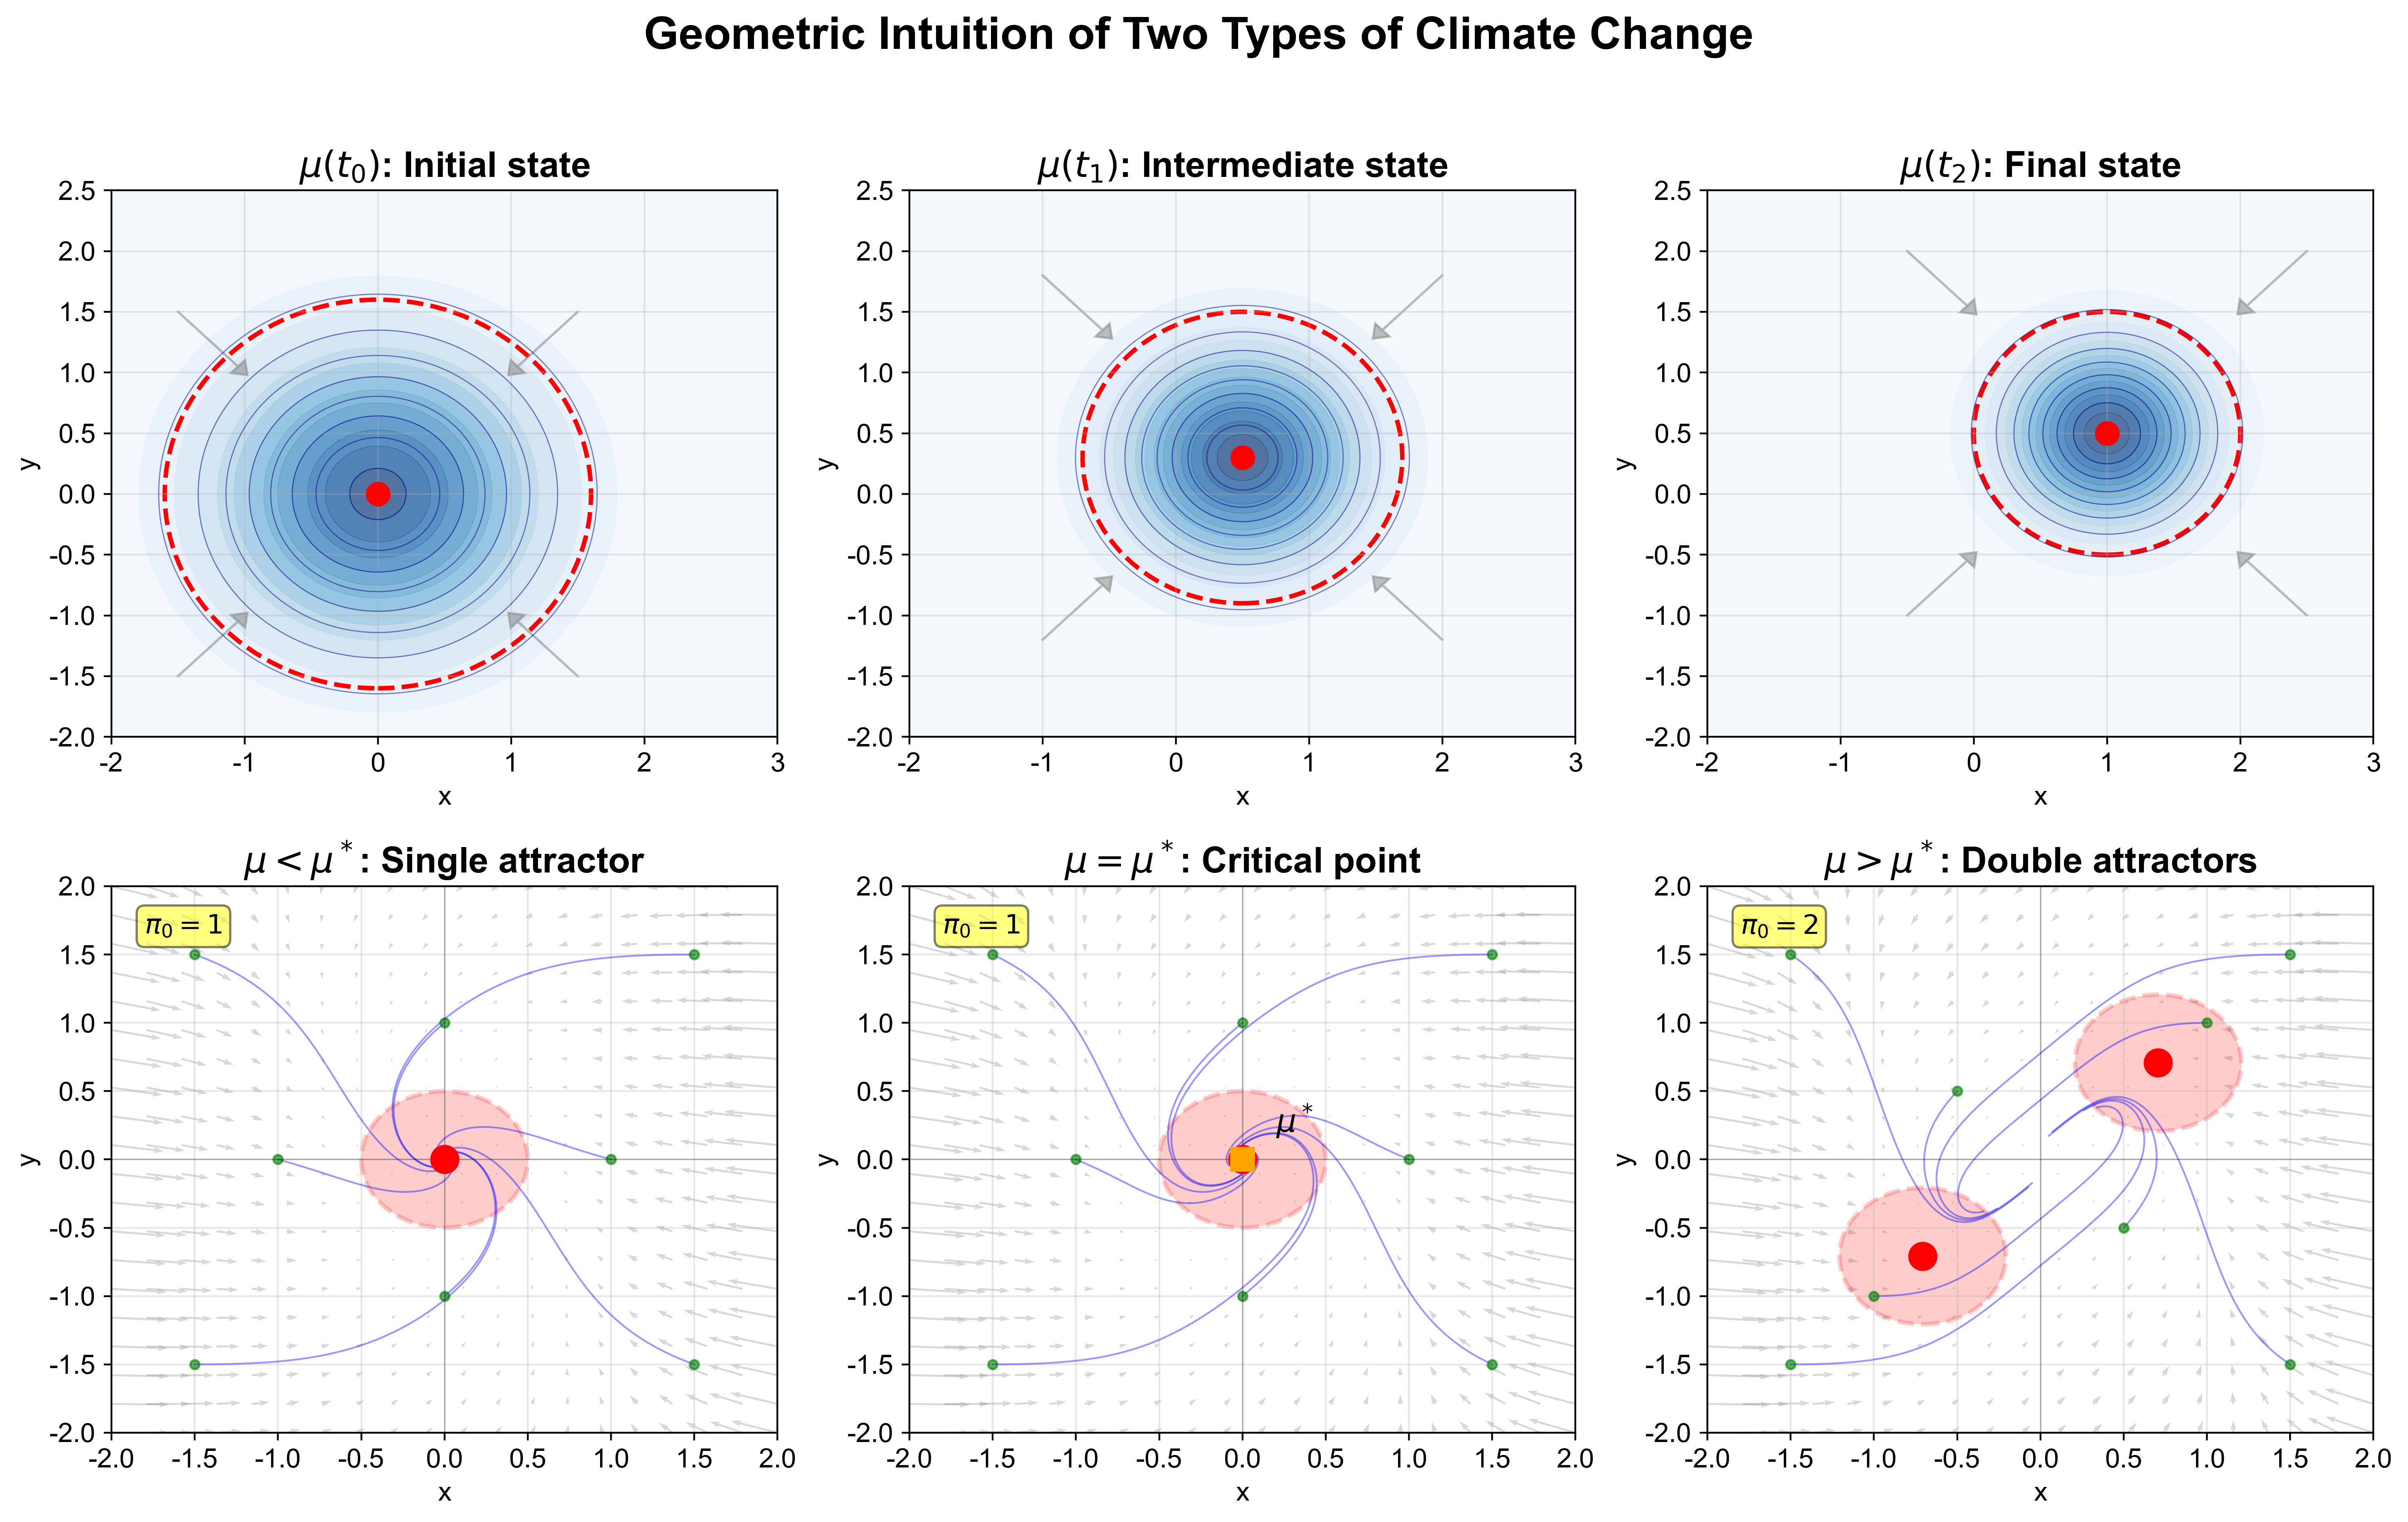
\includegraphics[width=0.9\textwidth]{./assets/climate_change_types.png}
    \caption{I类与II类气候变化的几何图景对比。上排: I类变化，吸引子 ($\pi_0 = 1$) 拓扑不变，概率测度在单个吸引子上重新分布，均值 $\mu$ 从 $\mu(t_0)$ 漂移到 $\mu(t_2)$。下排: II类变化，吸引子从单稳态 ($\pi_0 = 1$) 变为双稳态 ($\pi_0 = 2$)，产生了一个新的吸引子盆地，系统发生不可逆的跃迁。}
    \label{fig:climate_change_types}
\end{figure}

\subsection{I类气候变化: 概率测度的演化}

\begin{definition}[I类气候变化]
\label{def:type1_climate}
    若慢变量 $\slowvar(t)$ 在时间区间 $[t_0, t_1]$ 内演化，气候吸引子 $\attractor_{\slowvar(t)}$ 满足拓扑不变性:
    \begin{equation}
    \label{eq:type1_topology}
        H_*(\attractor_{\slowvar(t)}) \cong H_*(\attractor_{\slowvar(t_0)}), \quad \pi_0(\attractor_{\slowvar(t)}) = \text{const}, \quad \forall t \in [t_0, t_1]
    \end{equation}

    而流形度量 $\metric_{\slowvar(t)}$ 和概率测度 $\measure_{\slowvar(t)}$ 连续演化，则称系统发生I类气候变化。
\end{definition}

这里 $H_*$ 表示同调群 (Homology Groups)，$\pi_0$ 表示连通分量数 (Number of Connected Components)。
方程 \eqref{eq:type1_topology} 的数学意义是吸引子的个数和连通性保持不变。
原则上，I类变化具有可逆性: 若慢变量回复到初始值 $\slowvar(t_1) \to \slowvar(t_0)$，系统将回到初始气候状态。

\textbf{I类气候变化是当前气候系统的主要演化模式}。
其核心特征是概率测度 $\measure_{\slowvar}$ 随慢变量 $\slowvar$ 的演化。
我们首先说明，在I类变化中，吸引子拓扑保持不变，流形与度量的演化缓慢且效应不明显，但概率测度 $\measure_{\slowvar}$ 可以发生较显著的改变。

稳态Fokker-Planck方程 \eqref{eq:steady_fp} 的解 $\probdens_{ss}$ 由漂移向量场 $\drift$ 和扩散张量 $\difftensor$ 决定。
考虑一维系统 (可推广到高维情况)，不变概率测度满足 (参见 \cite{gardiner2009stochastic}):
\begin{equation}
\label{eq:steady_fp_solution}
    \probdens_{ss}(x; \slowvar) \propto \frac{1}{\difftensor(x; \slowvar)} \exp\left(\int^x \frac{2\drift(y; \slowvar)}{\difftensor(y; \slowvar)} dy\right)
\end{equation}

对 $\drift$ 求变分导数:
\begin{equation}
\label{eq:sensitivity_mean_partial_f}
    \frac{\delta \probdens_{ss}}{\delta \drift(z)} = \probdens_{ss}(x) \cdot \frac{2}{\difftensor(z)} \cdot H(x - z)
\end{equation}

其中 $H$ 是Heaviside函数。
因此:
\begin{equation}
    \frac{\partial \meanval}{\partial \drift(z)} = \int x \cdot \frac{\delta \probdens_{ss}}{\delta \drift(z)} dx = \frac{2}{\difftensor(z)} \int_{z}^{\infty} x \probdens_{ss}(x) dx \sim O(1/\difftensor)
\end{equation}

类似地，对 $\difftensor$ 求变分导数，可得:
\begin{equation}
    \frac{\partial \meanval}{\partial \difftensor(z)} \sim O(1/\difftensor^2), \quad \frac{\partial \sigma^2}{\partial \drift(z)} \sim O(1/\difftensor), \quad \frac{\partial \sigma^2}{\partial \difftensor(z)} \sim O(1/\difftensor^2)
\end{equation}

这表明，漂移向量场 $\drift$ 的微小改变 ($\Delta \drift$) 会导致均值和方差以 $O(1/\difftensor)$ 的速率变化；扩散系数 $\difftensor$ 的微小改变 ($\Delta \difftensor$) 会导致均值和方差以 $O(1/\difftensor^2)$ 的速率变化。
由于噪声强度 $\difftensor$ 相对较小，均值和方差对动力学参数的变化高度敏感。
微扰 ($\Delta \drift, \Delta \difftensor$) 将通过Fokker-Planck方程被“放大”为统计量的显著变化 ($\Delta \meanval, \Delta \sigma^2$)，这是\textbf{对气候变化非线性效应的动力学解释}。

概率测度 $\measure_{\slowvar}$ 的改变将对人类社会产生直接且重要的影响，尤其是尾部概率的变化，体现为\textbf{极端事件}频率的指数增长。

设 $\climind: \manifold \to \R$ 为气候指标 (温度、降水强度、风速等)，定义极端事件为 $\climind(\fastvar) > \threshold$，其中 $\threshold$ 为高阈值。
极端事件的发生概率由不变测度 $\probdens_{ss}$ 的尾部决定:
\begin{equation}
\label{eq:extreme_prob}
    P_{\text{extreme}}(\threshold; \slowvar) = \measure_{\slowvar}(\{\fastvar \in \manifold_{\slowvar} : \climind(\fastvar) > \threshold\}) = \int_{\climind(\fastvar) > \threshold} \probdens_{ss}(\fastvar; \slowvar) \, d\fastvar
\end{equation}

对应的\textbf{重现期 (Return Period)} 为:
\begin{equation}
\label{eq:return_period}
    T_{\text{return}}(\threshold; \slowvar) = \frac{1}{P_{\text{extreme}}(\threshold; \slowvar)}
\end{equation}

假设气候指标 $\climind(\fastvar)$ 近似服从正态分布:
\begin{equation}
\label{eq:normal_approx}
    \climind(\fastvar) \sim \mathcal{N}(\meanval(\slowvar), \sigma^2(\slowvar))
\end{equation}

其中 $\meanval(\slowvar) = \int \climind(\fastvar) \probdens_{ss}(\fastvar; \slowvar) d\fastvar$ 为均值；$\sigma^2(\slowvar) = \int (\climind(\fastvar) - \meanval)^2 \probdens_{ss}(\fastvar; \slowvar) d\fastvar$ 为方差。

对于高阈值 $\threshold \gg \meanval$，极端事件概率可用互补误差函数表示:
\begin{equation}
    \label{eq:extreme_prob_normal}
        P_{\text{extreme}}(\threshold; \slowvar) \approx \frac{1}{2}\mathrm{erfc}\left(\frac{\threshold - \meanval(\slowvar)}{\sqrt{2}\sqrt{\variance(\slowvar)}}\right) \sim \exp\left(-\frac{(\threshold - \meanval(\slowvar))^2}{2\variance(\slowvar)}\right)
    \end{equation}

慢变量变化 $\slowvar \to \slowvar'$ 导致概率测度的演化 $\measure_{\slowvar} \to \measure_{\slowvar'}$，从而改变均值 $\meanval$ 和方差 $\sigma^2$。
我们分别分析两种效应:

\textbf{(1) 均值漂移的影响}

若均值变化 $\meanval(\slowvar') = \meanval(\slowvar) + \Delta \meanval$ (不妨设 $\Delta \meanval > 0$)，方差不变，则尾部概率的相对变化为:
\begin{align*}
    \frac{P_{\text{extreme}}(\theta; \slowvar')}{P_{\text{extreme}}(\theta; \slowvar)} &= \exp\left(-\frac{(\theta - \meanval - \Delta\meanval)^2}{2\sigma^2} + \frac{(\theta - \meanval)^2}{2\sigma^2}\right) \\
    &= \exp\left(\frac{2(\theta - \meanval)\Delta\meanval - (\Delta\meanval)^2}{2\sigma^2}\right)
\end{align*}

当 $\Delta\meanval \ll \theta - \meanval$ 时，忽略二次项得:
\begin{equation}
\label{eq:extreme_prob_mean_shift}
    \frac{P_{\text{extreme}}(\threshold; \slowvar')}{P_{\text{extreme}}(\threshold; \slowvar)} \approx \exp\left(\frac{(\threshold - \meanval)\Delta \meanval}{\sigma^2}\right)
\end{equation}

由于 $\threshold \gg \meanval$，即使很小的均值变化 $\Delta \meanval$ 也会导致极端事件概率的显著增加。
取 $\theta - \meanval = 3\sigma$ (概率约千分之一)，若$\Delta\meanval = 0.1\sigma$，概率增加因子为 $\exp(3 \times 0.1) \approx 1.35$；若 $\Delta\meanval = \sigma$，增加因子将高达 $\exp(3) \approx 20$。

\textbf{(2) 方差增加的影响}

若方差变化 $\sigma^2(\slowvar') = \sigma^2(\slowvar) + \Delta \sigma^2$，均值不变，则尾部概率变化为:
\begin{equation*}
    \frac{P_{\text{extreme}}(\threshold; \slowvar')}{P_{\text{extreme}}(\threshold; \slowvar)} \approx \sqrt{\frac{\sigma^2}{\sigma^2 + \Delta\sigma^2}} \exp\left(\frac{(\threshold - \meanval)^2 \Delta \sigma^2}{2\sigma^2(\sigma^2 + \Delta\sigma^2)}\right)
\end{equation*}

当 $\Delta\sigma^2 \ll \sigma^2$ 时，主导项为:
\begin{equation}
\label{eq:extreme_prob_variance_increase}
    \frac{P_{\text{extreme}}(\threshold; \slowvar')}{P_{\text{extreme}}(\threshold; \slowvar)} \approx \exp\left(\frac{(\threshold - \meanval)^2 \Delta \sigma^2}{2(\sigma^2)^2}\right)
\end{equation}

方差增大将使概率测度尾部加厚 (Fat Tail)，分布更加扁平，极端值的概率密度更高。
由于 $\theta \gg \meanval$，即使方差的相对变化很小，极端事件概率也会显著增加。
若 $\theta - \meanval = 3\sigma$，方差增加 $10\%$ (即 $\Delta\sigma^2 / \sigma^2 = 0.1$)，概率增加因子约为 $\exp(9 \times 0.1 / 2) \approx 1.57$。

近年来，人类活动导致的气候变化已经导致了极端事件发生频率的极大提高。
以全球变暖为例，$\text{CO}_2$ 浓度从工业革命前的 $280$ ppm 升至当前的 $420$ ppm，全球温度均值升高约 $1.1$ °C，方差增加约 $15\%$ \cite{ipcc2021ar6}。
根据IPCC AR6报告 \cite{ipcc2021ar6}，$1.5$ °C的增温将使千年一遇的极端热浪变为百年一遇，重现期缩短10倍，对应概率增加10倍。
这正是均值漂移和方差增加带来的指数增长效应。

综上所述，我们从概率测度的角度定量分析了气候变化对极端事件概率的影响，揭示了动力学参数、概率测度和极端事件之间的关系链条:
\begin{equation*}
\Delta \drift, \Delta \difftensor \xrightarrow{\text{Fokker-Planck}} \Delta \meanval, \Delta \sigma^2 \xrightarrow{\text{尾部放大}} \Delta P_{\text{extreme}} \sim \exp(\cdot)
\end{equation*}

\subsection{II类气候变化: 拓扑突变与临界转变}

\begin{definition}[II类气候变化]
\label{def:type2_climate}
    若慢变量跨越临界值 $\slowvar^*$ 时，气候吸引子的拓扑结构发生间断改变:
    \begin{equation}
    \label{eq:type2_topology}
        H_*(\attractor_{\slowvar_-}) \not\cong H_*(\attractor_{\slowvar_+}), \quad \text{或} \quad \pi_0(\attractor_{\slowvar_-}) \neq \pi_0(\attractor_{\slowvar_+}), \quad \text{或} \quad \dim_H(\attractor_{\slowvar}) \text{跳跃}
    \end{equation}

    其中 $\slowvar_{\pm} = \slowvar^* \pm \epsilon$，则称系统发生II类气候变化，$\slowvar^*$ 为临界点 (Tipping Point)。
\end{definition}

II类变化对应动力系统的\textbf{分岔 (Bifurcation)}。
在临界点 $\slowvar^*$ 处，向量场 $\drift_{\slowvar}$ 的雅可比矩阵至少有一个特征值穿越虚轴 ($\mathrm{Re}(\eigenval) = 0$)，导致吸引子的稳定性发生质变。
常见的分岔类型包括:
\begin{enumerate}
    \item Saddle-node分岔: 其中吸引子与鞍点碰撞湮灭，系统跳跃到另一个吸引子 ($\pi_0: 2 \to 1$)；
    \item Hopf分岔: 稳定不动点失稳并产生极限环 (周期振荡)，拓扑维度增加 ($\dim_H: 0 \to 1$)；
    \item Pitchfork分岔: 单一吸引子分裂为两个对称吸引子，对称性自发破缺 ($\pi_0: 1 \to 2$)。
\end{enumerate}

\begin{figure}[htbp]
    \centering
    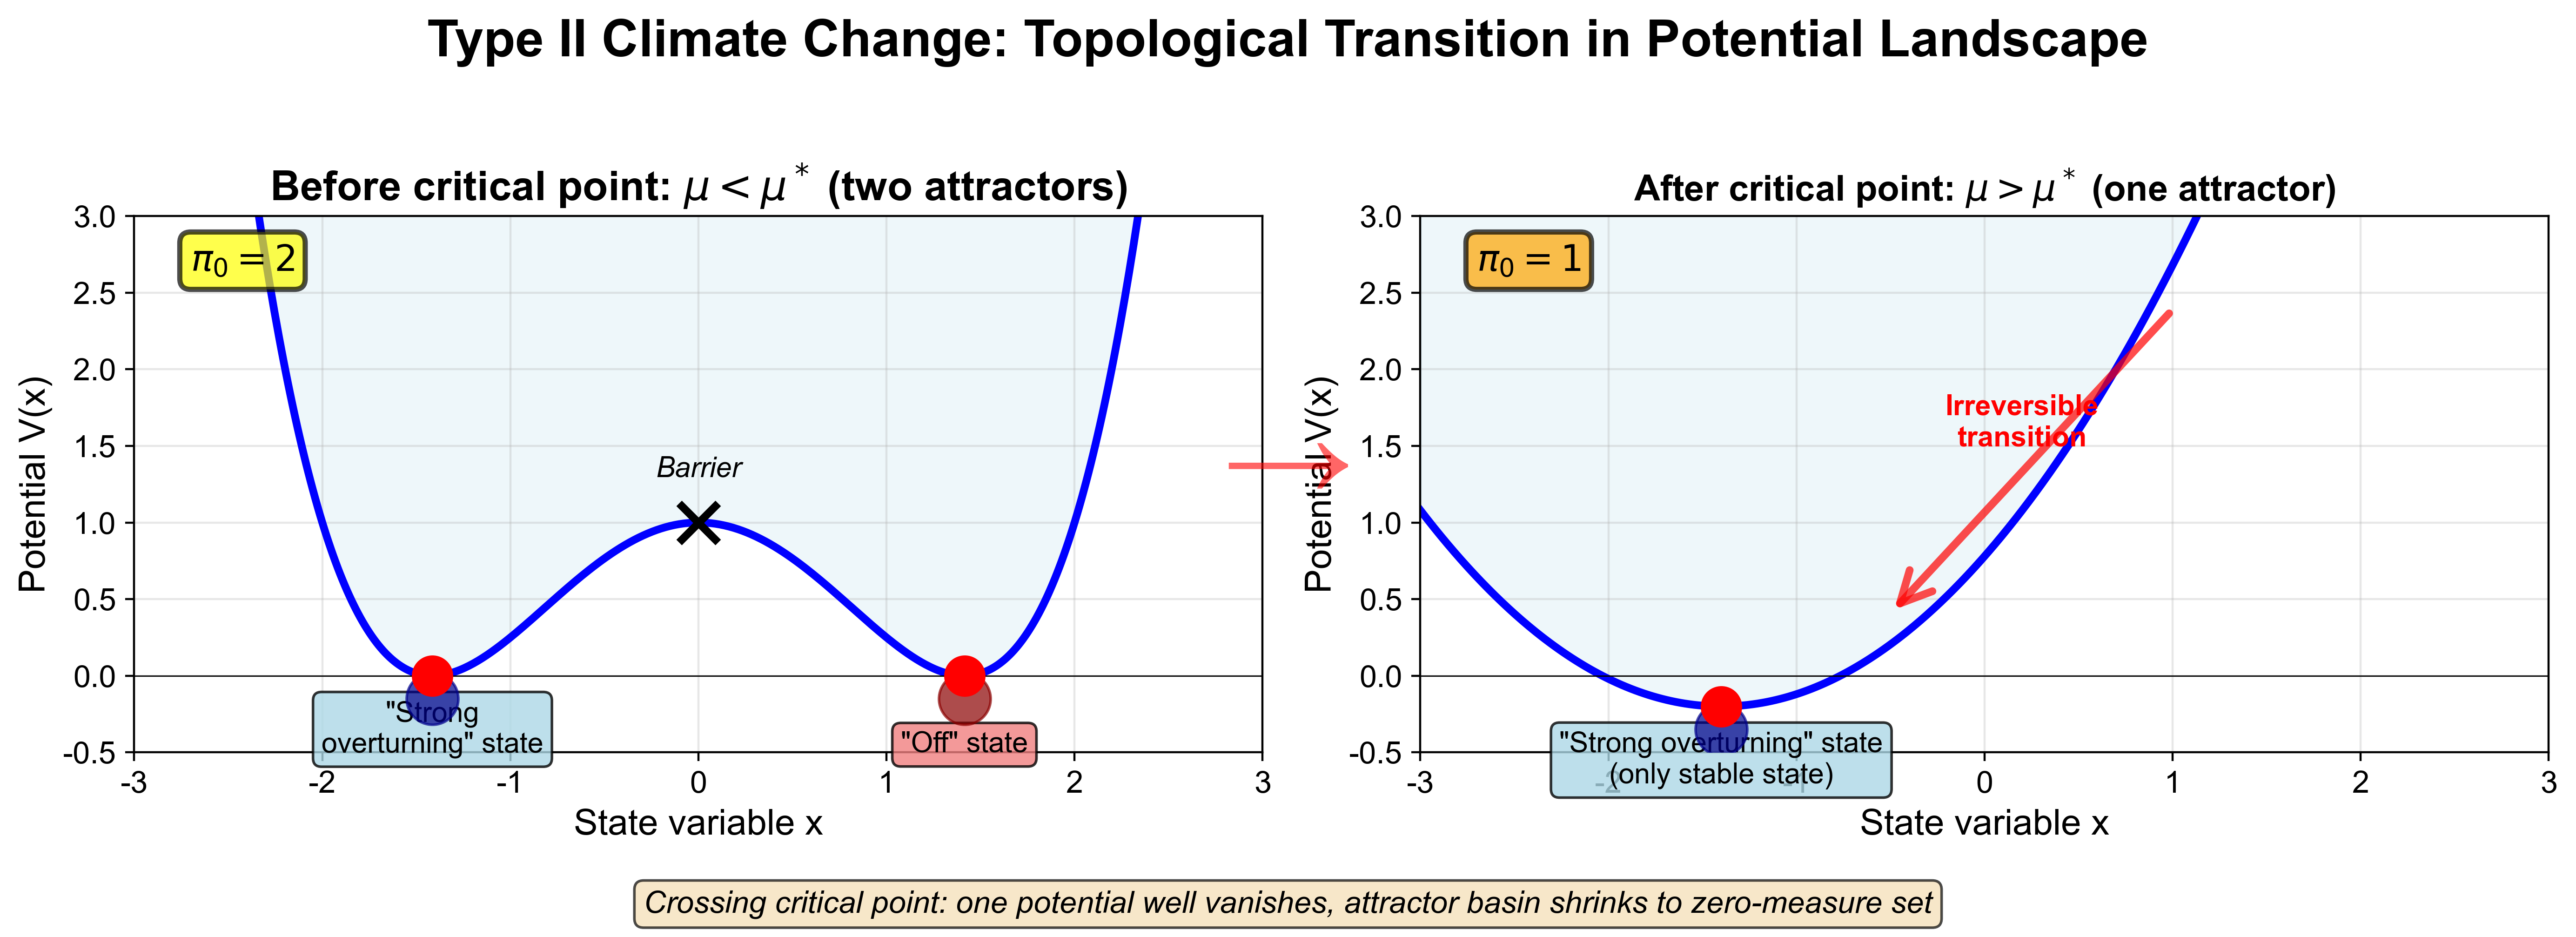
\includegraphics[width=1.00\textwidth]{./assets/potential_landscape_transition.png}
    \caption{Saddle-nod 分岔的势函数图景。左: 临界点前 ($\mu < \mu^*$)，双势阱对应两个吸引子 ($\pi_0 = 2$)态。右: 临界点后 ($\mu > \mu^*$)，右侧势阱消失，仅剩单一吸引子 ($\pi_0 = 1$)。}
    \label{fig:potential_landscape}
\end{figure}

II类变化的本质特征是不可逆性: 跨越临界点后，即使慢变量回复，系统也无法自动回到原来的吸引子，因为该吸引子已不复存在。

接近临界点时，系统将在多个层面呈现出可测量的\textbf{预警信号 (Early Warning Signals)} \cite{scheffer2009early}:
\begin{itemize}
    \item \textbf{临界慢化 (Critical Slowing Down)}:
    系统对扰动的恢复时间 $\predtime \sim 1/\sqrt{\eigenval} \to \infty$。
    具体表现为主导衰减模式的松弛率 $\eigenval_{\text{relax}} = -\mathrm{Re}(\eigenval_{\text{leading}}) \to 0^+$。
    \item \textbf{自相关增强 (Autocorrelation Enhancement)}:
    时间序列的滞后-1自相关系数趋近于1: $\mathrm{AC}(1) = \mathrm{Corr}(x_t, x_{t-1}) \to 1$，表明系统的“记忆”增强，状态转移减慢。
    临界点处 $\mathrm{AC}(1) \approx 1 - 2\eigenval_{\text{relax}}\Delta t$，可用于估计距临界点的距离。
    \item \textbf{方差发散}:
    概率测度向鞍点附近集中，导致状态变量的方差趋于无穷: $\mathrm{Var}[\fastvar] \to \infty$。
\end{itemize}

2009年，Rockström等学者提出了行星边界理论 (Planetary Boundaries theorem) \cite{rockstrom2009planetary}，认为地球系统存在9个临界子系统，即存在9个气候流形上的吸引子正在接近临界点 $\slowvar^*$。
这一理论为理解地球系统的稳态特性与气候变化的临界点提供了重要框架。

对于II类气候变化，我们介绍\textbf{大西洋经向翻转环流 (Atlantic Meridional Overturning Circulation, AMOC)} 的潜在崩溃作为典型案例。
AMOC是全球气候系统的关键组分，通过将热带暖水输送至北大西洋并驱动深层冷水南下，调节全球热量分布。
其驱动力来自北大西洋的密度差——表层海水在高纬度冷却增密并下沉，形成深层返流。然而，格陵兰冰盖融化释放的淡水正在降低海水盐度，从而减弱密度梯度并削弱环流强度。
当淡水通量超过临界阈值 $F^* \sim 0.1$ Sv时，系统将跨越临界点 \cite{stommel1961thermohaline,lenton2008tipping,dijkstra2005stability}。

从拓扑结构来看，AMOC存在两个吸引子态: “强翻转”态 ($\sim 20$ Sv，当前态) 和“弱翻转/关闭”态 ($< 5$ Sv)。
这对应两个独立的吸引子盆地 ($\pi_0 = 2$)。
临界点处，“强翻转”盆地在相空间中收缩至零测度集，随后消失 ($\pi_0: 2 \to 1$)，系统被迫不可逆跃迁至“关闭”态。
数学上，这是一个\textbf{Saddle-node分岔}，吸引子与鞍点在临界流形上碰撞湮灭。

观测数据为这一理论预测提供了有力支持。
Ditlevsen \& Ditlevsen (2023) \cite{ditlevsen2023warning} 分析了1870-2020年间的AMOC指标 (海温梯度、盐度剖面)，发现了多个临界预警信号。
自相关系数从1950年代的 $\mathrm{ACF}(1) \approx 0.7$ 增至2020年的 $\approx 0.9$，增幅达 $0.2$，这对应着松弛时间从 $20$ 年延长至 $100$ 年。
同时，方差增长率 $d\mathrm{Var}/dt > 0$ 且在1970年代后加速，符合临界慢化理论的预测。
基于这些信号，统计模型估计AMOC可能在2040-2070年间跨越临界点 ($95\%$置信区间)。

AMOC崩溃的全球影响将是灾难性的。
北欧地区将因失去暖流输送而温度下降 $3-5$ °C；热带辐合带将因大气环流重组而南移；美国东海岸将因海洋动力学高度变化而经历 $30-50$ cm的海平面上升；亚马逊和非洲萨赫勒地区将因远程气候耦合而降水减少 $20-40\%$。
这些变化对应着地球系统吸引子流形的拓扑重构，将影响数十亿人的生存环境 \cite{jackson2015global,ipcc2014ar5}。
\newpage

\bibliographystyle{unsrtnat}
\bibliography{references}

\end{document}
